%% Chapter 14 — 모니터링과 신뢰성
\setcounter{chapter}{13}
\chapter{모니터링과 신뢰성}
\chaptersubtitle{서빙 지표, Prometheus와 Grafana, 소진율 경보, 드리프트 — ssh로 감당할 수 없게 된 플릿의 관제 센터}

\begin{calloutbox}{tbbblue}{tbbbluefill}
{\normalsize\bfseries\color{tbbblue}학습 목표}\par\vspace{3pt}
\begin{tbbitemize}
  \item 겉으로 건강해 보이는 플릿이 사용자에게는 실패할 수 있는 이유를 설명하고, probe·log·평균·\code{nvidia-smi}가 각각 SLO와는 \textit{다른} 질문에 답한다는 사실을 이해한다.
  \item 세 가지 지표 형태(counter, gauge, histogram), node·cAdvisor·kube-state·DCGM·engine \code{/\allowbreak metrics}로 이어지는 exporter 생태계, percentile을 \textit{올바르게} 집계하는 PromQL을 사용해 서빙 플릿 전체를 계측한다.
  \item 약속, 누구, 이유, 기반의 네 행으로 서빙 dashboard를 설계해 49분짜리 수색을 두 번의 시선으로 끝내는 진단으로 바꾼다.
  \item SLO 문장을 \textbf{소진율 경보}(여러 window, page와 ticket 구분)로 바꾸고, 올바른 이유로 올바른 사람만 깨우는 경보 목록을 설계한다.
  \item Canary도 page도 볼 수 없는 느린 실패인 \textbf{드리프트}를 분포 검사(PSI), 플릿이 이미 내보내는 sentinel metric, 관찰에서 재학습까지 이어지는 대응 사다리로 감지한다.
  \item Dashboard가 답하는 runbook, registry 항목에 연결한 비난 없는 postmortem, 모든 개선의 가치를 수치화하는 MTTD/MTTR로 전체 신뢰성 순환 고리를 운영한다.
\end{tbbitemize}
\end{calloutbox}

\vspace{2.5pt}

\begin{calloutbox}{tbbteal}{tbbtealfill}
{\normalsize\bfseries\color{tbbteal}핵심 용어}\par\vspace{3pt}
모니터링과 관측 가능성 · 세 기둥(metric · log · trace) · exporter · scrape · 시계열 · cardinality · counter / gauge / histogram · le bucket · PromQL · rate() · histogram\_quantile() · recording rule · ServiceMonitor · DCGM · kube-state-metrics · RED / USE 방법 · 네 행 dashboard · 증상과 원인 · 오류 예산 · 소진율 · 여러 window 경보 · 경보 피로 · dead man’s switch · synthetic probe · data / concept drift · PSI · sentinel metric · MTTD / MTTR · 비난 없는 postmortem
\end{calloutbox}

\vspace{2.5pt}

\begin{calloutbox}{tbblightgray}{tbbboxfill}
{\normalsize\bfseries\color{tbbink}이 장의 구성}\par\vspace{3pt}
\textbf{14.1} 두 번의 밤, 하나의 플릿, 그리고 아무도 몰랐던 스위치    \textbf{14.2} 지표: 플릿을 정직하게 계측하기    \textbf{14.3} Prometheus와 Grafana: 실제 네 행 dashboard    \textbf{14.4} 경보: page, 소진율, 거짓 경보를 피하는 기술    \textbf{14.5} 드리프트: 절대 page를 울리지 않는 실패    \textbf{14.6} 실습: 관제 센터를 만들고 두 번 깨뜨리기. 이어서 요약, 연습문제, 더 읽을거리를 다룬다.
\end{calloutbox}

\section{두 번의 밤, 하나의 플릿, 그리고 아무도 몰랐던 스위치}

제13장은 promotion과 조용한 경고로 끝났다. Canary의 analysis loop는 30분 동안 "TTFT가 정직한가? 행동이 drift했는가?"라는 정확한 질문을 던진 뒤 꺼졌지만, production은 \textit{아무도 듣지 않는 곳에서 영원히} 그 질문에 답하고 있었다. 이 장에서는 그 답을 들을 청중을 만든다. 제12장이 외상으로 남겨 둔 전쟁 이야기도 있다(§12.4: "SLO 아래의 time-slicing은 p99 미스터리가 태어나는 방식이다. 제14장에서 그중 하나를 만난다"). 이제 그 빚을 갚는 밤에서 시작하자. v9-int4의 canary가 끝난 지 3주 된 어느 화요일이다. 오늘 배포된 것은 없고, 아침과 똑같은 L4 레플리카 네 대가 실행 중이다. 21:30에 cluster 어딘가에서 예약 job이 시작되고, 22:06에 pager가 아니라 support 전화가 on-call을 깨운다. 아직 pager가 없기 때문이다.

\begin{terminalbox}
\begin{Verbatim}[breaklines=true,breakanywhere=true,fontsize=\small,formatcom=\color{tbbtermfg},codes=\tbbcodeactive]
# tuesday 22:06. "chat is molasses." uptime checker: /health 200 OK,
# green all night. no deploy since friday. so... what changed?
$ kubectl get pods -l app=chat
#   chat-1..chat-4  Running  READY 1/1  RESTARTS 0   <- reflexes: fine
$ kubectl logs deploy/chat --since=30m | grep -ci error
#   0                                                <- nothing confessed
$ curl -s chat-1:8000/metrics | grep ttft   # spot-check... ONE pod
#   p99 0.44 s. fine?!            <- you sampled a healthy replica
$ python mean_latency.py --since 21:00
#   mean e2e 15.2 s -> 21.3 s (+40%). "users exaggerate."
# 22:29  ssh gpu-node-2; nvidia-smi: util 93%, mem 21.9/24 GiB
#        "busy = evening peak, right?"      <- util counts ANYONE's kernels
# 22:33  wrong fix: scale to 6 replicas (150 s births). p99 -> 2.9 s.
#        better! not fixed. (the sick replica still serves 1 in 6.)
# 22:47  nvidia-smi once more, slower this time: TWO python processes
#        on one GPU. the 12.4-lab time-slice config, still on the node.
#        eval-nightly has been sharing chat-2's card since 21:30.
# 22:55  eval job killed. p99 0.46 s. total: 85 bad user-minutes.
\end{Verbatim}
\end{terminalbox}
\figcaption{사례 14-A  앞을 보지 못한 첫째 밤. 모든 도구가 정직하게 답했지만 질문이 모두 틀렸다. Probe는 약속이 아니라 생존을 확인하고, log는 침묵이 아니라 고백만 기록한다. 평균은 고통받은 사용자 4분의 1을 숨기며, pod 하나의 /metrics는 일화에 불과하다. GPU “utilization”은 누구의 것이든 kernel을 센다. 전화가 울리고 49분 뒤, 누군가 §12.4 실험을 기억해 낸 덕분에 마침내 원인을 찾았다.}

이 사례의 잔인함에는 배울 점이 있으니 잠시 곱씹어 보자. \textbf{거짓말한 것은 하나도 없었다.} Pod는 정말 Ready였다. Readiness는 반사 작용이고(제5장), process는 느린 batch 사이사이에 probe에 응답했다. Log도 정말 깨끗했다. Engine은 error를 내는 대신 \textit{기다리고} 있었고, 기다림은 log를 남기지 않는다. 평균도 실제로 40\%만 늘었다. 제7장에서 \textbf{평균은 아무도 묘사하지 않는다}고 경고했듯, 여기서는 건강한 레플리카 세 대와 물에 빠진 한 대를 섞어 버렸다. Curl로 확인한 \code{/\allowbreak metrics} endpoint의 p99도 정말 0.44초였다. 우연히 살아남은 레플리카를 골랐을 뿐이며, 어차피 레플리카별 percentile의 평균으로 플릿 전체를 설명할 수 없다(§14.2에서 정확히 살펴본다). \code{nvidia-smi}도 실제로 utilization 93\%를 표시했다. 다만 card에 상주하는 \textit{누군가의} kernel을 셀 뿐 \textit{누구의 것인지}는 말하지 않는다. 참인 문장 다섯 개, 진단은 0개다. 부족했던 것은 정직함이 아니라 \textbf{조립}이었다. SLO가 정의한 "정상"을 계속 계산하고 레플리카별로 분해해, 그 이유를 설명하는 계층 바로 위에 한눈에 놓는 장소가 필요했다. 그 장소에는 이름이 있다. 같은 화요일을 그 장소와 함께 다시 재생하면 처음부터 끝까지 20분이면 된다.

\begin{terminalbox}
\begin{Verbatim}[breaklines=true,breakanywhere=true,fontsize=\small,formatcom=\color{tbbtermfg},codes=\tbbcodeactive]
# the same tuesday, replayed with mission control (this week's lab).
# 21:31  slack #serving-alerts  [severity: ticket]
#        DuplicatePodsOnProdGPU: uuid GPU-...3d9f hosts 2 pods
#        (chat-2, eval-nightly-28471)          runbook R7
# 21:42  phone  [severity: page]
#        QueueSustained: num_requests_waiting > 8 for 5m on chat-2
#        (chat-1/3/4: 0)                       runbook R2 -> row 3
# 21:44  the walk (Figure 14-4): row 2 -> chat-2 only, LB fair;
#        row 3 -> decode step 2.1x, queue local, KV normal;
#        row 4 -> GPU ...3d9f: two pods. there is the neighbor.
# 21:47  kubectl delete job eval-nightly    # + incident note -> registry
# 21:50  queue drained. p99 0.46 s. page auto-resolves.
#        two-line diagnosis: "chat-2 only; shared GPU."
#        20 bad user-minutes, 8 of them yours. same on-call, same brain.
\end{Verbatim}
\end{terminalbox}
\figcaption{사례 14-B  둘째 밤. 이 장의 장치를 갖춘 뒤 같은 플릿에서 똑같은 사고가 일어났다. 21:31의 ticket은 사용자가 증상을 느끼기 전에 원인을 지목했고, 21:42의 page에는 runbook이 붙어 있었다. Dashboard는 진단을 번호가 붙은 순서로 바꾸었다. 두 밤 사이에 사람이 더 똑똑해진 것은 아니다. 질문을 미리 해 두었을 뿐이다.}

\begin{tbbfigure}
  \adjustbox{max width=0.94\linewidth,max totalheight=0.46\textheight}{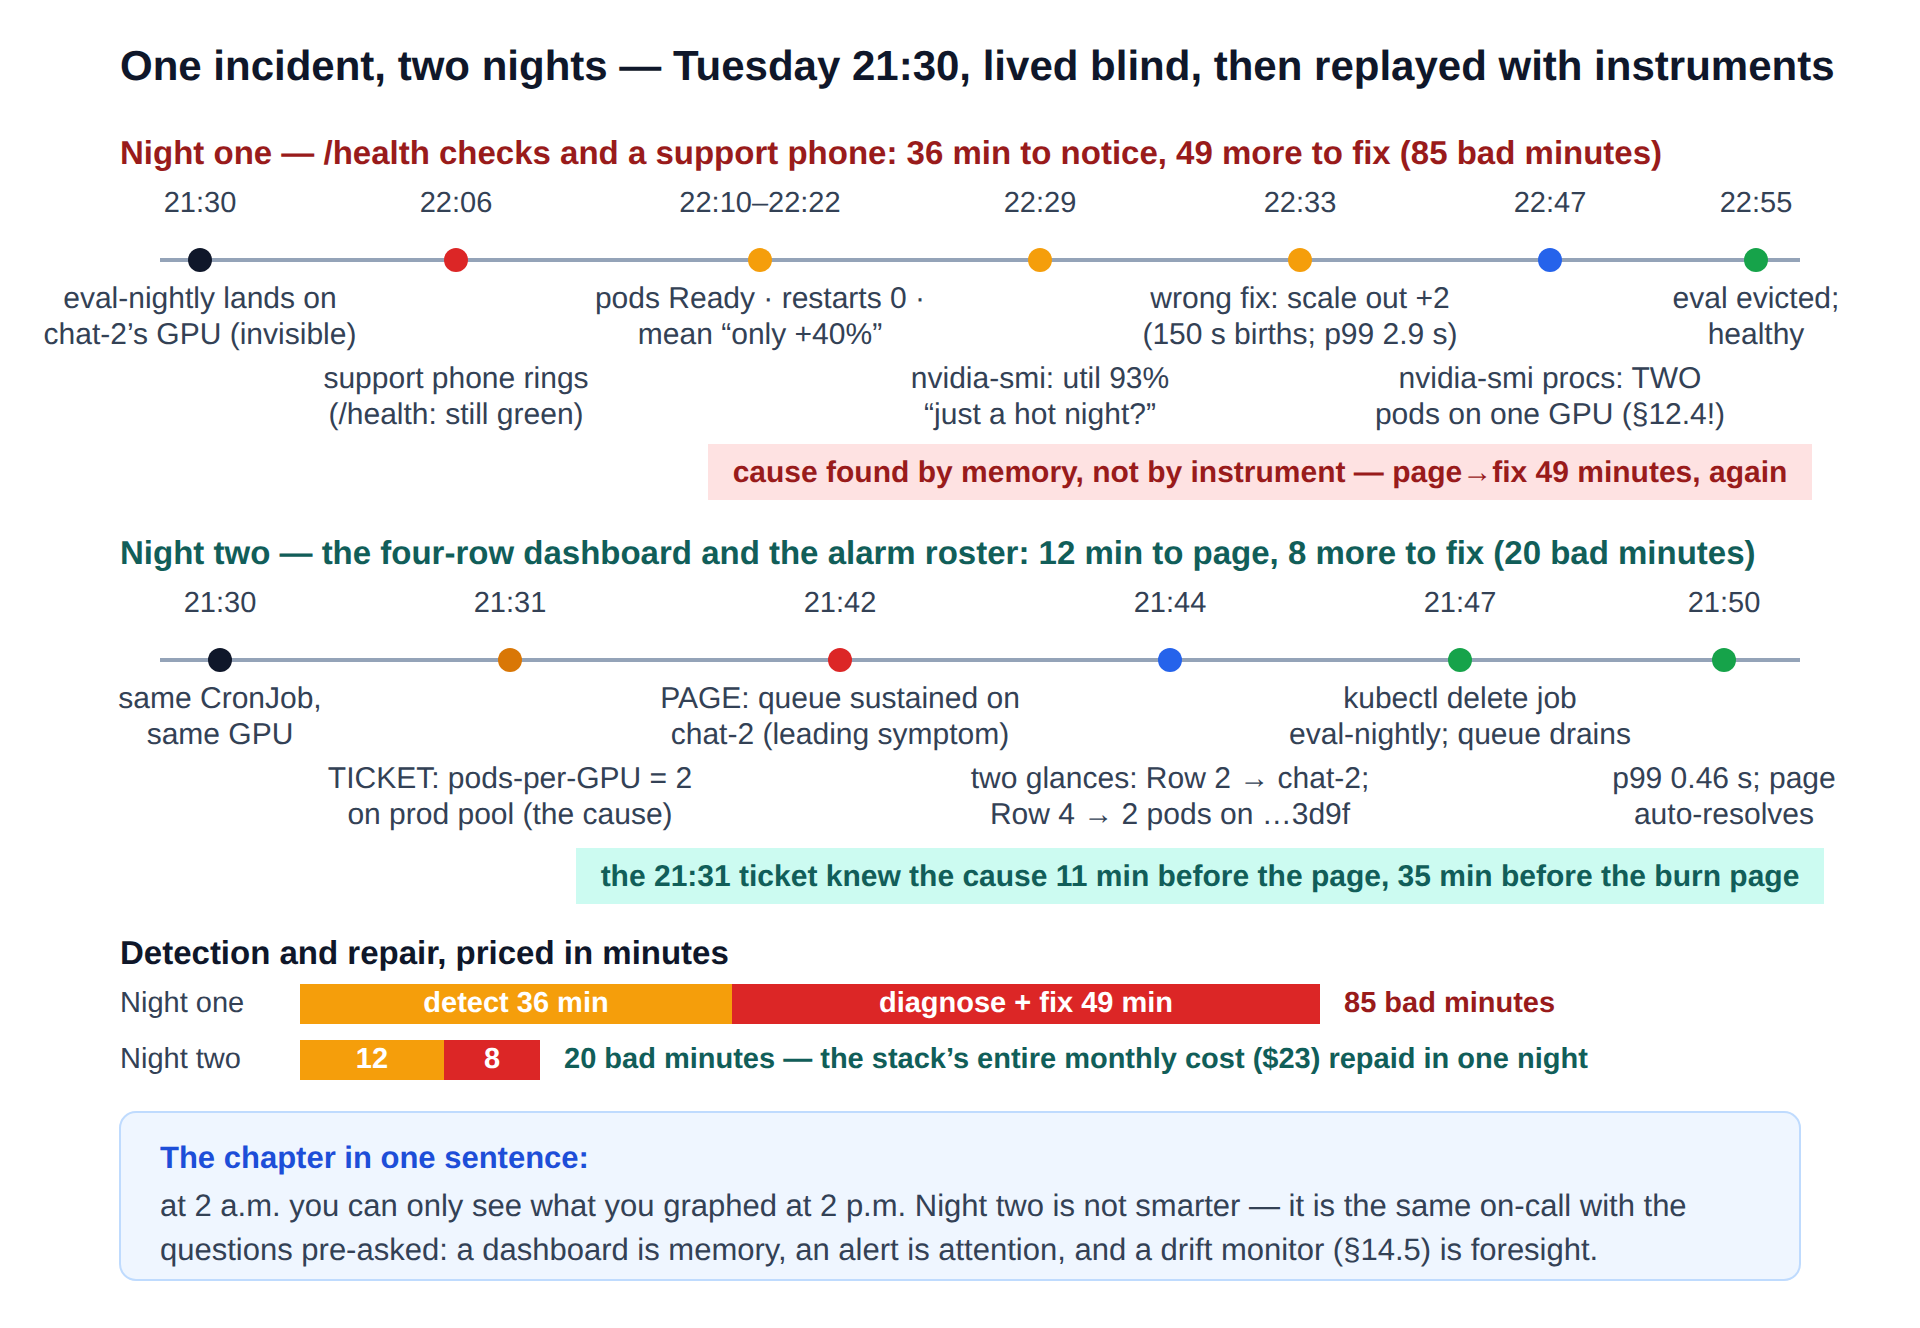
\includegraphics{figures/fig14-1_twonights.png}}\\[3pt]
  \figcaption{그림 14-1  한 사고를 겪은 두 번의 밤. 첫째 밤에는 support를 통해 알아차리는 데 36분, 도구를 하나씩 발굴하는 데 다시 49분이 걸렸다. 나쁜 시간 85분 뒤 기억에 의존해 원인을 찾았다. 둘째 밤에는 21:31에 원인을 ticket으로 알리고, 21:42에 증상을 page로 보내, 21:50에 고쳤다. 나쁜 시간은 20분이었다. 두 행 사이의 거리가 바로 이 장이다.}
\end{tbbfigure}

\subsection*{1969년 11월 14일: telemetry가 엉망이 되었고, 한 관제사는 그 모습을 본 적이 있었다}

Apollo 12가 비 내리는 Florida에서 이륙한 지 36.5초 뒤, 번개가 Saturn V를 때렸다. Capsule 안에서는 fuel cell offline과 bus 저전압을 비롯한 panel의 모든 경고등이 한꺼번에 켜졌고, Houston 관제사의 화면은 잡음이 섞인 의미 없는 숫자로 무너졌다. Commander는 그것이 무엇을 뜻하는지 모른 채 침착하고 전문적인 목소리로 panel을 지상에 읽어 주었다. 16초 뒤 두 번째 번개가 상황을 더 악화했다. 이미 시야 밖으로 사라진 vehicle을 볼 수 있는 유일한 수단인 telemetry가 알아볼 수 없는 상태에서, 관제 센터는 2분 안에 달 착륙 임무를 중단할지 결정해야 했다. 그때 24세 비행 관제사 \textbf{John Aaron}이 우주 비행 역사에서 가장 유명한 문장 가운데 하나를 말했다. \textit{“Flight, try SCE to Aux.”} Flight director도 astronaut도 그 방의 어느 누구도 이 switch를 알지 못했다. 1년 전 화려할 것 없는 pad test에서 Aaron은 telemetry가 \textit{정확히 같은 형태}로 무너지는 모습을 보았고, 근무 외 시간에 원인을 추적해 Signal Conditioning Equipment라는 잘 알려지지 않은 box를 찾아냈다. Auxiliary power mode로 바꾸면 문제가 해결된다는 것도 알아냈다. Lunar module pilot Alan Bean이 switch를 찾았고 telemetry가 즉시 돌아왔다. Fuel cell을 reset한 뒤 임무는 달을 향해 계속되었으며, Aaron은 모든 운영 엔지니어가 남몰래 부러워할 별명인 \textit{the steely-eyed missile man}을 얻었다.

이 장의 모든 가르침이 그 90초 안에 있다. \textbf{첫째, telemetry는 미리 설계하지 않으면 존재하지 않는다.} Saturn V가 수천 channel을 지상으로 전송한 이유는 rocket에 ssh로 접속할 수 없음을 엔지니어들이 받아들였기 때문이다. 자기 플릿도 autoscaling node의 레플리카 네 대가 되는 날 같은 선을 넘었다. 사례 14-A는 그 규모에서 "직접 걸어가 확인하는 일"의 비용이다. \textbf{둘째, 원시 signal은 시야가 아니다.} 그 2분 동안 Houston에는 data가 있었다. 임무를 구한 것은 전에 본 적 있고 이름이 붙었으며 행동과 연결된 \textit{알아볼 수 있는 signature}였다. Dashboard가 정확히 그런 역할을 한다. Aaron이 SCE의 엉망인 pattern을 알아본 것처럼 화요일의 on-call이 "레플리카 하나는 빨강, GPU 하나에 pod 둘"을 알아보도록 signature를 미리 그려 둔다. \textbf{셋째, 알아보는 능력은 drill에서 산다.} Aaron은 위기 때가 아니라 \textit{test}에서 실패를 보았다. 그래서 이 장의 실습은 dashboard를 열어 둔 채 자기 플릿에서 사례 14-A를 일부러 재현하며 끝난다. NASA는 simulation, 제13장은 두 번 깨뜨리기, SRE 문헌은 game day라고 부른다. 이름보다 중요한 것은 일정에 넣는 일이다. Apollo에는 1202 alarm, 손으로 쓴 cheat sheet, 좋은 paging 정책의 기원이라는 두 번째 교훈도 있지만 §14.4에서 다룬다.

\subsection*{모니터링, 관측 가능성, 세 기둥 — 비용으로 이해하는 용어}

도구에 앞서 용어부터 정리하자. \textbf{모니터링}은 미리 정한 signal을 계속 수집하고 기대와 비교하는 활동이다. p99가 500 ms 아래인가, queue가 얕은가, budget이 소진되는가처럼 \textit{물어야 한다고 알고 있던} 질문에 답한다. \textbf{관측 가능성}은 밖으로 드러나는 signal을 이용해 미리 정의하지 \textit{않은} 질문에 답할 수 있는 system의 성질이다. 둘째 밤의 "레플리카 하나만 느린 이유는 무엇인가?"는 어느 runbook 제목에도 없었지만 레플리카별 queue, decode step time, GPU별 pod를 \textit{조합}해 두 번의 시선으로 답을 만들 수 있었다. 서로 독립적이고 label이 붙은 signal을 충분히 내보내 관측 가능성을 사고, 이미 아는 signal을 dashboard와 alarm에 연결해 모니터링을 수행한다. 업계는 둘을 \textbf{세 기둥}으로 제공하며, 무엇을 고를지는 비용의 형태로 정직하게 판단해야 한다(그림 14-2). \textbf{Metric}은 source에서 집계한 label이 붙은 숫자다. Token counter, queue depth gauge, TTFT histogram이 예다. Event마다 increment 한 번이면 되므로 비용이 거의 없고 traffic volume이 커져도 그대로 버티며, \textit{상시} 평가할 만큼 저렴한 유일한 기둥이다. 그래서 alert와 이 장이 metric에 자리 잡는다. \textbf{Log}는 event마다 남기는 기록, 즉 pod의 전기다. 이상하게 동작한 요청 하나를 찾는 데 꼭 필요하고 volume에 비례해 비용이 든다. 제5장의 entourage가 log shipper를 약속했고 실습에서 request\_id를 담은 구조화 JSON을 보내도록 설치한다. \textbf{Trace}는 요청 하나가 service를 지나는 경로를 따라 hop별 시간을 기록한다. Microservice debugger의 기둥이지만 event당 가장 비싸므로 sampling한다. 40개 service를 지나는 결제 경로와 달리 네 hop짜리 serving 경로는 그만큼 필요하지 않아 이 과정에서는 §14.2의 OpenTelemetry 한 문단으로 제한한다. 세 기둥을 묶는 규칙은 제6장에서 이미 비용을 냈다. \textbf{Telemetry는 pod 밖으로 계속 보낸다.} Pod가 죽기 직전 몇 분은 바로 그 pod가 직접 이야기할 수 없는 시간이기 때문이다. 제3장의 OOM kill은 app log가 아니라 cgroup counter와 event에 증거를 남겼다.

제5장은 이 장과 probe를 구분하는, 새겨 둘 만한 문장을 주었다. \textbf{Probe는 반사 작용이고 모니터링은 기억이다.} Liveness probe는 hang이 나면 restart하는 행동만 하고 설명하지 않는다. Readiness는 traffic을 차단하는 행동만 하고 설명하지 않는다. 화요일 내내 process가 살아서 응답했으므로 둘 다 초록색이었다. 모니터링 자체는 설명만 할 뿐 행동하지 않는다. System의 기억(21:35의 queue는 어땠는가?), 주의력(기억을 전화 진동으로 바꾸는 alert), §14.5의 drift detection을 더하면 예지력(현실이 어느 방향으로 벗어나는가?)이 된다. 성숙한 플릿에는 두 신경계가 모두 필요하다. 제5장의 논술은 관측 가능성 없는 reconciliation이 자기가 고친 일을 감추는 \textit{사고 억압}이라고 경고했다. 이번 주에는 Kubernetes가 조용히 모으던 restart counter, OOM event, endpoint 공백이 모두 graph와 alert가 되는 선으로 바뀐다. Drift correction의 \textit{빈도}를 chart에 그려야 90초마다 한 번씩 restart를 일으킬 만큼 작게 잡힌 limit를 발견할 수 있다.

앞으로 90분 동안 갈 길을 살펴보자. \textbf{§14.2}에서는 세 가지 metric 형태, node부터 DCGM과 engine의 \code{/\allowbreak metrics}까지 이어지는 exporter 생태계(마침내 graph가 되는 제11장의 줄), 플릿 규모에서 percentile을 올바르게 계산하는 두 가지 PromQL 주문으로 signal 계층을 만든다. \textbf{§14.3}에서는 약속, 누구, 이유, 기반으로 이루어진 \textbf{네 행 dashboard}를 조립하고, 그 위에서 panel을 하나씩 따라 둘째 밤을 재생해 §12.4의 빚을 모두 갚는다. \textbf{§14.4}에서는 \textbf{alarm}을 연결한다. SLO 문장을 burn rate로 compile하고, 빠른 소진은 page로, 느린 소진은 ticket으로 보내는 여러 window 정책을 만들며, 증상과 원인을 구분해 routing한다. 거부할 수 있는 모든 계층의 바깥에서 synthetic probe를 실행하고(마침내 감시받는 제6장의 문), 감시자를 감시하는 dead man’s switch를 더한다. Runbook, on-call, 비난 없는 postmortem으로 이어지는 사람의 순환 고리도 다룬다. \textbf{§14.5}에서는 절대 page를 울리지 않는 실패인 \textbf{드리프트}를 살펴본다. 제13장의 canary가 구조적으로 잡을 수 없는 경사면을 손으로 계산할 수 있는 PSI와 플릿이 이미 무료로 내보내는 sentinel로 찾는다. \textbf{§14.6}은 강의계획서가 약속한 serving dashboard와 alarm 구축 실습에, 강의계획서가 좀처럼 약속하지 않는 부분을 더한다. 두 번 깨뜨리고 자기 panel이 그것을 잡게 한다. 관제 센터를 세운 뒤 임무를 수행한다.

\begin{calloutbox}{tbbpurple}{tbbpurplefill}
{\normalsize\bfseries\color{tbbpurple}생각해 보기}\par\vspace{3pt}
\begin{tbbitemize}
  \item 사례 14-A의 on-call은 다섯 가지를 확인했고 모두 “정상”이라는 답을 얻었다. Probe, log, 평균 latency, pod 하나의 /metrics, nvidia-smi util이 \textbf{실제로} 답하는 질문과 SLO 문장이 답해야 했던 질문을 각각 말하자. 그림 14-4의 panel 하나로 다섯 가지를 모두 대신한다면 어느 것인가?
  \item 22:33의 “잘못된 해결책”, 즉 레플리카를 6대로 늘린 조치는 p99를 실제로 4.6초에서 2.9초로 개선했다. 제12장의 산술을 이용해 레플리카 추가가 아픈 레플리카 하나의 영향을 희석할 뿐 치료하지는 못하는 이유를 설명하자. 진단을 가리는 동안 추가 레플리카 두 대의 시간당 비용은 얼마였는가?
  \item John Aaron의 해결에는 (a) 이상 중에도 계속 흐른 telemetry, (b) drill에서 본 signature, (c) 실제로 존재한 switch가 필요했다. 세 가지를 둘째 밤에 대응시키고, 자기 프로젝트 플릿에서 가장 가능성 높은 실패에 대비할 때 지금 빠진 것이 무엇인지 밝히자.
  \item 둘째 밤에는 원인 alert(21:31, ticket)가 증상 alert(21:42, page)보다 먼저 왔다. 심각도를 반대로 배정하지 않은 이유를 설명하자. 원인처럼 보이는 모든 이상이 page를 울리면 on-call의 삶은 어떻게 되는가? 답은 잠시 보류하자. §14.4에서 병원 통계로 비용을 계산한다.
\end{tbbitemize}
\end{calloutbox}

\section{지표: 플릿을 정직하게 계측하기}

\textbf{지표(metric)}는 시스템이 자신에 관해 말할 수 있는 가장 작고 정직한 문장이다. \textit{이름}, \textit{레이블} 집합, \textit{숫자}, \textit{시각}으로 이루어진다. \code{vllm:num\_requests\_waiting\{pod="chat-2"\} 19 @21:41:30}에는 주어, 한정어, 서술어, 타임스탬프가 모두 들어 있다. 이 장의 모든 내용은 이런 문장을 15초마다 수집하고 몇 주 동안 보관한 뒤, 집계해서 질의하는 데서 출발한다. 이름과 레이블의 조합이 하나씩 달라질 때마다 별도의 \textbf{시계열(time series)}이 생긴다. 이 분야의 첫 번째 법칙은 관측값이 아니라 \textit{시계열} 단위로 비용을 치른다는 것이다. 값이 네 개인 레이블(파드)은 지표 하나를 네 시계열로 늘릴 뿐이라 괜찮다. 값이 900만 개인 레이블(사용자 ID나 요청 ID)은 이를 900만 시계열로 늘린다. 이것은 모니터링의 탈을 쓴 메모리 장벽이다. 비용을 감당하려면 다음 규칙을 지켜야 한다. \textbf{레이블은 한정된 목록에서 “어느 것인가?”에 답해야 한다.} 파드, 모델, GPU UUID, 경로가 그 예다. 값의 수가 무한히 늘어날 수 있는 정보는 로그에 두어야 한다. 로그는 이벤트별 저장이 재앙이 아니라 애초의 설계이기 때문이다. (이 강좌의 플릿에는 약 14,000개의 활성 시계열이 있다. 그림 14-2에서 대략 계산한 값으로, 초당 표본은 약 1,000개이고 15일 보존 기간에 필요한 공간은 2GB 미만이다. 부주의하게 \code{user\_id} 레이블 하나만 추가해도 이 수가 천 배로 늘어난다.)

\begin{tbbfigure}
  \adjustbox{max width=0.94\linewidth,max totalheight=0.46\textheight}{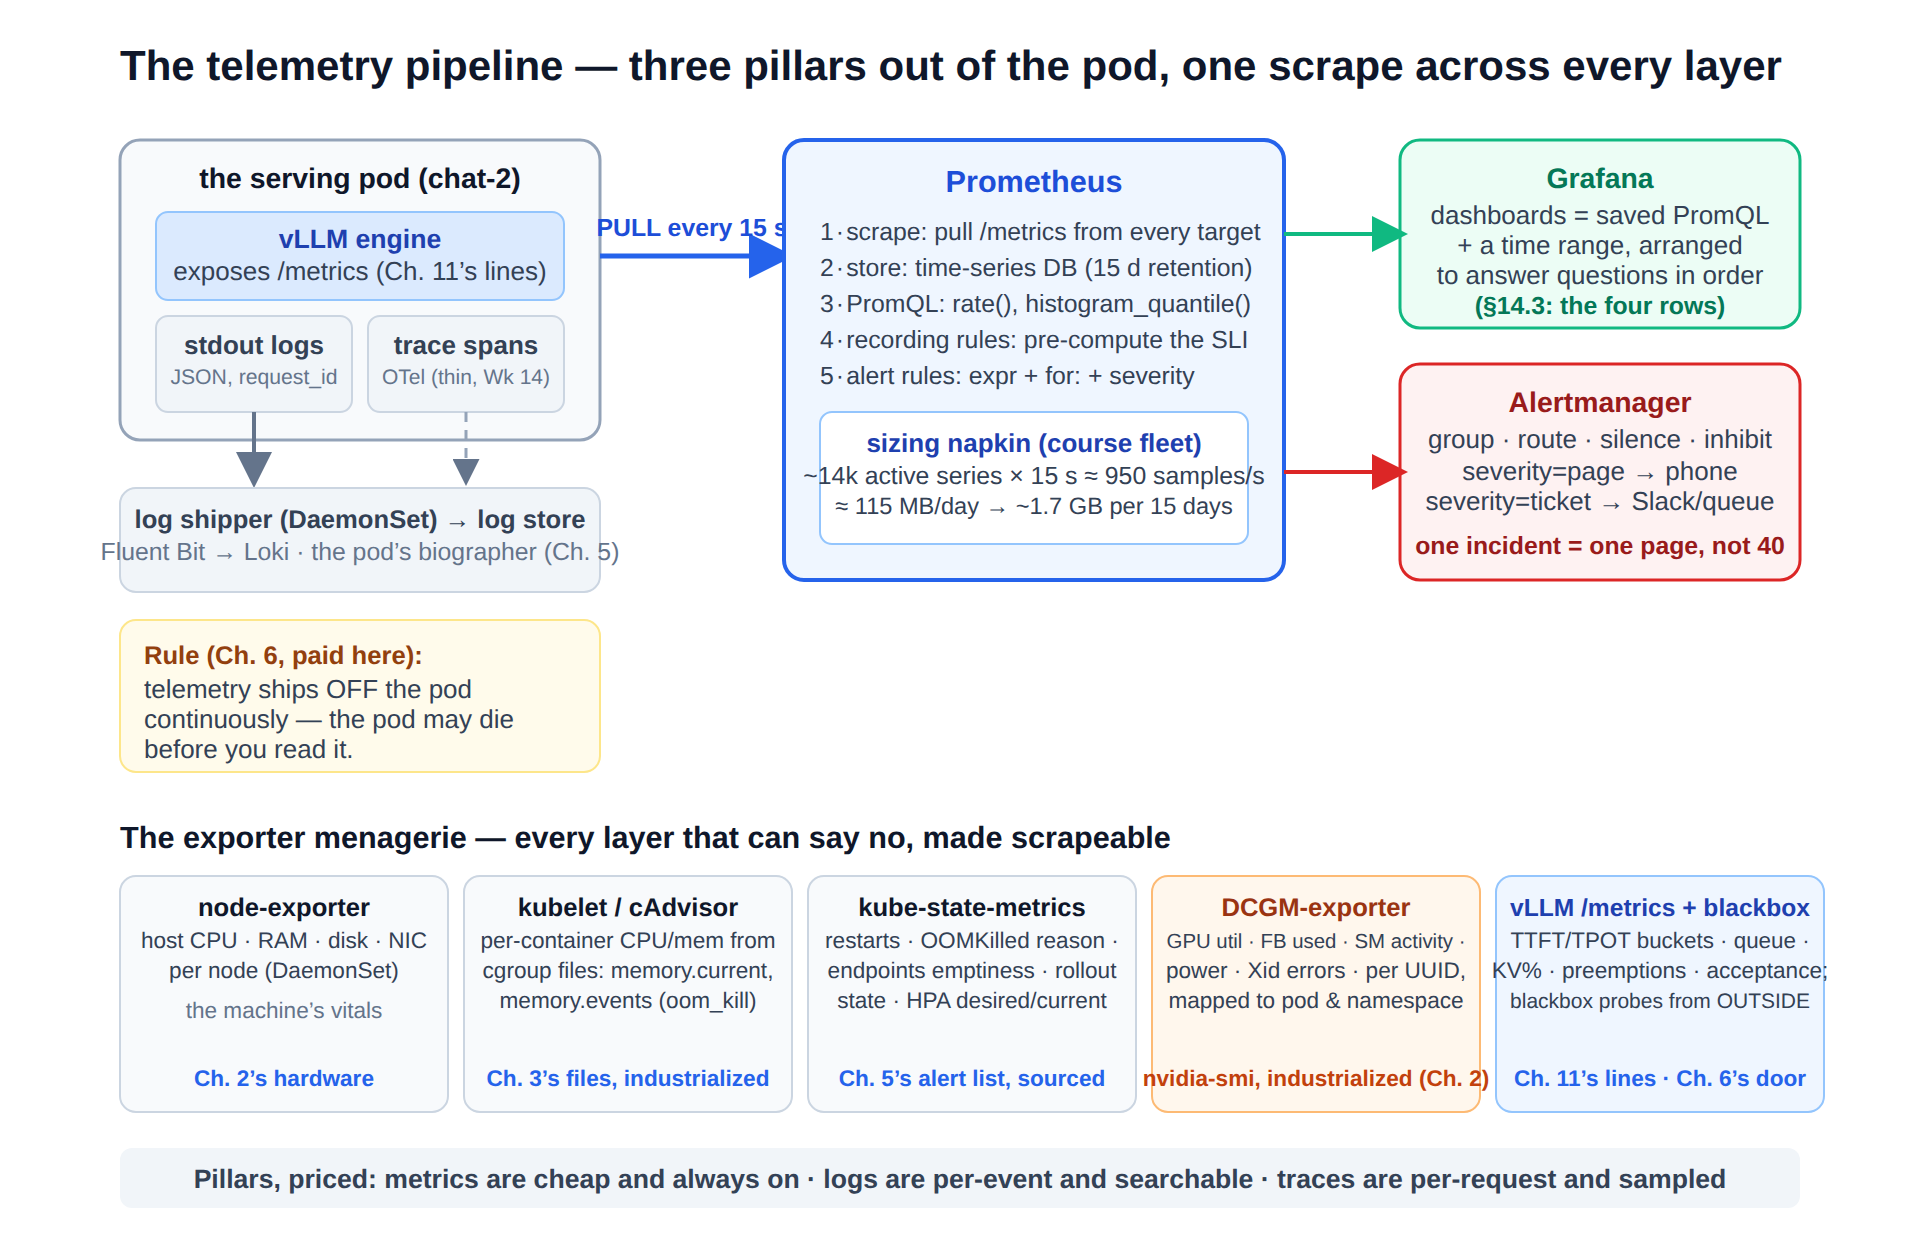
\includegraphics{figures/fig14-2_pipeline.png}}\\[3pt]
  \figcaption{그림 14-2  텔레메트리 파이프라인. Prometheus가 모든 계층에서 지표를 가져와 Grafana(질문)와 Alertmanager(호출)로 나누어 보낸다. 로그는 기록되는 즉시 DaemonSet을 통해 전송하고, 이 강좌에서는 트레이스를 최소한으로 유지한다. 아래쪽에는 여섯 관측 지점의 익스포터가 있다. 하나의 스크레이프 루프가 거부할 수 있는 모든 계층을 수집 가능한 대상으로 만든다.}
\end{tbbfigure}

\subsection*{세 가지 형태: 카운터, 게이지, 히스토그램 — 세 번째가 이 강좌를 움직이는 이유}

내보내는 지표는 모두 세 형태 가운데 하나이며, 처음 배울 때 가장 흔한 실수는 형태를 잘못 고르는 것이다. \textbf{카운터}는 생성된 토큰 수, 부팅 이후의 선점 횟수, 완료된 요청 수처럼 오르기만 한다. 순간값 자체는 별 의미가 없다(선점 1,841회라고 해도 \textit{언제부터} 센 값인가?). 신호가 되는 것은 \textbf{변화율}이다. 그래서 질의 언어에서 가장 자주 쓰는 함수가 \code{rate(x[5m])}이다. 일정 구간의 초당 기울기를 계산하며, 재시작에도 안전하다. 파드가 다시 태어나면서 카운터가 0으로 초기화되면 이를 감지해 이어 계산한다. 직접 만든 “이번 분의 요청 수” 게이지보다 카운터를 선호해야 하는 이유가 하나 더 생긴다. \textbf{게이지}는 대기열 깊이, KV 캐시 점유율, 온도처럼 오르내리는 값이다. 게이지는 그대로 읽고, 파드나 시간에 걸쳐 \code{max}/\code{avg}로 집계하며, 포화 신호를 표현하기에 알맞다. 가장 흥미로운 것은 \textbf{히스토그램}이다. 히스토그램은 임곗값 이하의 관측값 개수를 세는 \textit{누적 버킷}(\code{le="0.25"}, \code{le="0.5"}, ...) 묶음과 누적 합계 및 개수로 구성된다. 이는 7장에서 남긴 문제를 정확히 해결하려고 존재한다. \textbf{백분위수는 평균을 내거나 더할 수 없다.} 레플리카 열 개의 p99를 어떤 방식으로 계산해도 플릿의 p99가 되지 않는다. 반면 버킷 \textit{카운터}는 다른 카운터처럼 더할 수 있다. 레플리카 네 개의 \code{le="0.5"} 버킷을 합치면 플릿 전체 분포를 얻고, 여기에서 원하는 분위수를 구할 수 있다. 히스토그램은 7장의 문법 규칙을 데이터 구조로 구현한 것이다.

실제 시스템에서 세 형태를 살펴보자. 11주차부터 실행해 온 엔진은 줄곧 세 형태를 모두 내보내고 있었다.

\begin{terminalbox}
\begin{Verbatim}[breaklines=true,breakanywhere=true,fontsize=\small,formatcom=\color{tbbtermfg},codes=\tbbcodeactive]
$ curl -s chat-2:8000/metrics | grep -E 'vllm:' | head -14
vllm:num_requests_running{model="chat-v9"} 32.0     <- gauge: the seats,
vllm:num_requests_waiting{model="chat-v9"} 19.0        full (11.3); and THE
vllm:gpu_cache_usage_perc{model="chat-v9"} 0.96        alarm line (11.4)
vllm:num_preemptions_total{model="chat-v9"} 1841.0  <- counter: rate() it
vllm:spec_decode_draft_acceptance_rate{...} 0.74    <- gauge: 11.5's bet,
                                                       still paying
vllm:time_to_first_token_seconds_bucket{le="0.25"} 811021.0   <- histogram:
vllm:time_to_first_token_seconds_bucket{le="0.5"}  947210.0      cumulative
vllm:time_to_first_token_seconds_bucket{le="1.0"}  951003.0      buckets
vllm:time_to_first_token_seconds_bucket{le="+Inf"} 953882.0      (le = "at
vllm:time_to_first_token_seconds_count 953882.0                  or below")

$ curl -s gpu-node-2:9400/metrics | grep -E 'DCGM' | head -3
DCGM_FI_DEV_GPU_UTIL{UUID="GPU-...3d9f",pod="chat-2"} 93
DCGM_FI_DEV_FB_USED{UUID="GPU-...3d9f",pod="chat-2"} 22429
DCGM_FI_DEV_XID_ERRORS{UUID="GPU-...3d9f"} 0
\end{Verbatim}
\end{terminalbox}
\figcaption{실행 기록 14-1  주석을 단 두 번의 스크레이프. 엔진은 세 형태를 모두 내보낸다. 전체 누적 요청 953,882개 가운데 947,210개의 TTFT가 0.5 s 이하였다는 점에 주목하자. 99.3\%로, SLO 자체의 SLI가 두 버킷 카운터에 그대로 드러나 있다. DCGM은 실리콘의 상태를 말해 준다. GPU UUID를 레이블로 삼고, 장치 플러그인 매핑을 거쳐 파드 레이블도 붙인다. 바로 이 조인이 화요일의 문제를 푼다.}

왜 \textbf{풀(pull)} 방식일까? Prometheus는 푸시를 받지 않고 대상을 스크레이프한다. 이는 배관 방식이 아니라 철학의 선택이다. 풀 방식에서는 수집 대상을 \textit{열거}할 수 있다. 서버는 Kubernetes에서 실시간으로 발견한 대상 목록을 보유한다. 따라서 “어떤 레플리카가 존재하는가?”와 “어떤 레플리카가 응답을 멈췄는가?”가 같은 사실이 된다. 스크레이프할 때마다 \code{up\{pod=...\}} 시계열을 기록하므로, 사고 도중 죽은 파드는 아무도 알아채지 못하는 침묵 대신 \code{up == 0}이라는 묘비를 남긴다. 푸시 시스템에서는 부재를 별도로 모델링해야만 알아낼 수 있다. 풀 방식은 계측 로직도 단순하게 유지한다. 엔진은 HTTP로 텍스트만 제공하면 되고, 지연 시간에 민감한 프로세스 안에 버퍼링, 배치 처리, 역압 로직을 넣지 않아도 된다. 그 대가로 Prometheus가 대상에 \textit{도달}할 수 있어야 하지만, 단일 클러스터 안에서는 문제가 되지 않는다. 이 설계에는 계보가 있다. Google 내부의 \textbf{Borgmon}은 5장에 나온 Borg와 비슷한 2003년 무렵 탄생해 화이트박스 \code{/\allowbreak varz} 엔드포인트, 중앙 풀러, 레이블 시계열용 질의 언어, 질의로 정의한 경보라는 패턴을 세웠다. 전 Google 엔지니어 Matt T. Proud와 Julius Volz는 2012년 SoundCloud에 합류한 뒤 이와 견줄 만한 공개 시스템이 없다는 사실을 알고 이를 오픈소스로 다시 만들었다. \textbf{Prometheus}는 2015년에 공개되었고 Cloud Native Computing Foundation의 두 번째 프로젝트가 되었다. 첫 번째는 Kubernetes였다. 두 프로젝트가 나란히 선택되었다는 사실은 업계가 이 둘을 한 설계의 두 절반으로 받아들였음을 보여 준다. \textbf{Grafana}는 반대편에서 출발했다. Torkel Ödegaard는 2014년에 로그 검색 UI인 Kibana 3를 포크해 범용 시계열 대시보드로 바꾸었다. 실습에서 설치하는 스택은 이 두 계보가 합류한 결과다.

\subsection*{네 가지 질의로 익히는 PromQL — 화요일의 문제를 푼 두 질의까지}

PromQL은 레이블이 붙은 시계열에 적용하는 집합대수처럼 읽힌다. 플릿 운영에 필요한 관용 패턴은 열두 개 남짓이면 충분하다. 다음 네 가지는 이 장을 떠받치는 핵심 질의다. 그중 가운데 두 개에는 그림 14-3의 교훈이 담겨 있으며, 사고가 난 구간에 실행한 결과를 보여 준다.

\begin{terminalbox}
\begin{Verbatim}[breaklines=true,breakanywhere=true,fontsize=\small,formatcom=\color{tbbtermfg},codes=\tbbcodeactive]
# 1. the WRONG fleet p99 (tuesday, 21:44) -- averaging per-replica p99s:
> avg( job:vllm_ttft:p99_5m )
2.76                    # experienced by nobody (Figure 14-3)

# 2. the RIGHT fleet p99 -- merge bucket counters, THEN take the quantile:
> histogram_quantile(0.99,
    sum by (le) (rate(vllm:time_to_first_token_seconds_bucket[5m])))
9.08                    # the promise, actually broken

# 3. decompose: waiting or working? (Ch. 9's split, per replica)
> max by (pod) (vllm:num_requests_waiting)
{pod="chat-1"} 0   {pod="chat-2"} 19   {pod="chat-3"} 0   {pod="chat-4"} 0
> histogram_quantile(0.5, sum by (pod, le)
    (rate(vllm:time_per_output_token_seconds_bucket[5m])))
{pod="chat-2"} 0.150    # vs 0.070 fleet norm: decode itself is 2.1x slower

# 4. the SLI as a ratio -- the number 14.4 will set on fire:
> sum(rate(vllm:time_to_first_token_seconds_bucket{le="0.5"}[5m]))
  / sum(rate(vllm:time_to_first_token_seconds_count[5m]))
0.762                   # 76.2% good this window; target 0.990
\end{Verbatim}
\end{terminalbox}
\figcaption{실행 기록 14-2  사고 구간에 실행한 네 가지 질의. 질의 1은 그럴듯하지만 틀린 답이다. 질의 2는 7장의 규칙을 기계로 실행한다. 질의 3은 “대기 중”과 “처리 중”을 분리한다. 9장에서 이 진단 정보만으로 대시보드 설계의 절반이 완성된다고 약속했다. 질의 4는 §14.4에서 소진율 호출로 변환할 SLI 비율이다.}

질의 2의 구조를 안쪽부터 한 번만 읽어 보면 완전히 이해할 수 있다. \code{rate(...bucket[5m])}는 각 누적 버킷 카운터를 초당 흐름으로 바꾼다. \code{sum by (le)}는 \textit{버킷 경계를 보존하면서} 레플리카별 흐름을 합친다. 분포를 여러 레플리카에 걸쳐 집계할 때 수학적으로 허용되는 유일한 방법이다. 이어서 \code{histogram\_quantile(0.99, ...)}가 합쳐진 버킷을 따라가 99번째 백분위수를 찾고, 해당 버킷 안에서 보간한다. 그래서 결과의 정밀도는 버킷 너비에 좌우된다. 실습에서 엔진 버킷 경계를 SLO \textit{바로 그 값}에 두는 이유도 여기에 있다. 경계를 정확히 0.5 s에 두면 p99 추정값은 여전히 근사치여도 SLI 비율은 정확해진다. 이제 한 가지 관용 패턴을 더 이름 붙일 차례다. \textbf{기록 규칙(recording rule)}은 Prometheus가 일정에 따라 질의를 다시 실행하고 그 결과를 새 시계열로 저장하는 규칙이다. 질의 4에는 \code{job:slo\_ttft\_good:ratio\_rate5m}를 만들고, 대시보드용으로는 파드마다 \code{job:vllm\_ttft:p99\_5m}를 만든다. 패널과 경보는 새로 고칠 때마다 원시 버킷을 다시 집계하지 않고 미리 계산된 결과를 읽는다. 규칙은 저장소의 YAML로 관리하며, 13장 이후의 모든 것과 마찬가지로 PR 검토를 받는다.

\subsection*{익스포터 모음 — 여섯 관측 지점과 각각의 역할}

Prometheus 자체는 아무것도 측정하지 않는다. 온도계를 들고 있는 것은 \textbf{익스포터}다. 그림 14-2 아래쪽의 익스포터 모음은 이 강좌의 스택을 마지막으로 한 번 더 관통한다. DaemonSet으로 실행되는 \textbf{node-exporter}는 CPU, 메모리, 디스크, 네트워크처럼 2장에서 다룬 머신 하드웨어를 시계열로 말해 준다. kubelet에 내장된 \textbf{cAdvisor}는 \textit{3장에서 직접 읽었던 바로 그 파일}, 즉 cgroup의 \code{memory.current}, \code{memory.events}, CPU 사용량 정보를 읽어 모든 컨테이너의 상태를 말한다. 여기서 3장의 두 교훈이 결실을 맺는다. 첫째는 정직한 마운트에 관한 주석이다. 컨테이너 안의 프로세스가 \code{/\allowbreak proc}를 조회하면 컨테이너가 아니라 \textit{호스트의} CPU와 메모리를 본다. 단순한 컨테이너 내부 에이전트가 거짓말하는 이유이며, cAdvisor가 대신 바깥에서 cgroup 트리를 읽는 이유다. 둘째는 경보다. \code{memory.events}는 \code{high}와 \code{oom\_kill} 경계를 넘은 횟수를 센다. 따라서 3장 실습에서 \code{memory.high}로 설계한 벽 직전의 경고 단계는 이제 Grafana가 그래프로 그리고 §14.4가 종료 코드 137이 나타나기 \textit{전에} 티켓을 만들 수 있는 카운터가 된다. 이 종료 코드는 마지막으로 한 번 더 레이블 값으로 등장한다. \textbf{kube-state-metrics}는 컨트롤 플레인의 \textit{의도}를 말한다. 재시작 횟수, 마지막 종료 원인인 \code{OOMKilled}, 배포에서 원하는 레플리카 수와 사용 가능한 레플리카 수의 차이, 비어 있는 엔드포인트, HPA 상태를 제공한다. “가용성만이 아니라 드리프트 교정 빈도에도 경보를 걸라”던 5장의 목록이 이제 데이터 원천을 얻는다. \textbf{DCGM-exporter}는 \code{nvidia-smi}를 산업 규모로 만든 도구다. 이는 2장의 약속대로 GPU UUID별 사용률, 프레임버퍼, 전력, 클록, Xid 오류 코드를 제공하고, 장치 플러그인 매핑으로 파드 이름과 조인한다. 덕분에 화요일의 문제는 표를 한 번 조회하는 일로 바뀌었다. 또한 “사용률”이 회피하는 질문에 답하는 프로파일링 계열(\code{DCGM\_FI\_PROF\_SM\_ACTIVE}, 텐서 파이프 활동)도 제공한다. 이 거짓말은 잠시 뒤 자세히 살펴본다. \textbf{엔진 자체의 /metrics}는 이미 확인했다. 여기에 9장에서 분류기 서비스가 제공한 Triton 카운터도 더하자. 이 카운터는 대기열 시간과 계산 시간을 이미 분리해 준다. \textbf{블랙박스 익스포터}는 \textit{바깥에서} 조사한다. 게이트웨이의 공개 출입구로 HTTP GET을 보내고, TCP 핸드셰이크를 수행하고, 스트리밍 토큰을 확인한다. 6장에서 사용자와 파드 사이의 모든 계층이 저마다의 방식으로 거부할 수 있음을 배웠기 때문이다. 플릿 내부에서만 자신을 측정하면 로드 밸런서 상태 확인이 실패하는 동안에도 플릿은 결백하다고 주장한다. 실행 기록 6-11의 교훈처럼 증거는 클러스터 밖에 있었다. 합성 검사는 §14.4에서 다루며, 익스포터는 그 결과를 시계열로 바꾸는 수단이다.

이제 22시 29분에 마주한 거짓말을 살펴보자. \code{nvidia-smi}가 출력하는 값과 같은 \code{DCGM\_FI\_DEV\_GPU\_UTIL}은 단 하나의 질문에만 답한다. \textit{최근 시간 가운데 누구의 것이든 커널 하나 이상이 장치에 올라와 있던 비율은 얼마인가?} 이 값은 \textbf{이진 점유 듀티 사이클}이지, 여유 용량이나 효율, 소유권을 측정한 값이 아니다. 작은 커널 하나를 계속 올려 두는 메모리 병목 디코드 루프는 ALU의 10분의 1만 사용하면서도 90\% 이상으로 표시된다. 10장의 루프라인이 대시보드의 함정으로 다시 나타난 것이다. 두 테넌트가 카드 하나를 시분할하면 각자 절반의 작업만 처리하면서도 \textit{둘 다} 값을 100\% 가까이 끌어올린다. 그 숫자만으로는 \textit{누구의} 커널인지도 알 수 없다. 첫날 밤 당직자는 93\%를 보고 “바쁘다, 그러므로 부하가 걸렸다, 그러므로 정상이다”라고 판단했다. 근거 없는 추론을 세 번 연달아 한 셈이다. GPU에 관해 정직한 질문을 던지고 정직한 데이터 원천에서 답을 구해야 한다. \textit{실리콘이 제값을 하고 있는가?}는 10장에서 예상한 값과 \code{PROF\_SM\_ACTIVE}, 텐서 파이프 활동을 비교해 답한다. \textit{메모리가 장벽인가?}는 디코드 중 \code{PROF\_DRAM\_ACTIVE}가 포화에 가까우면 메모리 장벽이 눈앞에 드러난다. \textit{카드가 정상인가?}는 Xid 오류, 온도, 전력을 본다. \textit{누구의 것인가?}는 4행의 결정적 증거인 UUID당 파드 조인으로 답한다. 사용률은 “무언가 달라졌다”는 신호로 쓸 만하므로 대시보드에 남긴다. 그러나 이 값만으로는 아무 호출도 보내지 않는다. 실습의 JSON에는 이 패널 아래에 늘 다음 캡션이 붙는다. \code{busy ≠ yours ≠ efficient}

이런 익스포터 모음을 정리하는 두 약어가 있으며 면접에서도 자주 등장한다. \textbf{RED}는 Rate, Errors, Duration의 약자로, 사용자가 호출하는 대상마다 행 하나를 두는 \textit{서비스 측} 관점이다. 초당 요청 수, 실패 비율, 지연 시간 분포를 본다. \textbf{USE}는 Utilization, Saturation, Errors의 약자로, 서비스가 소비하는 자원마다 행 하나를 두는 \textit{자원 측} 관점이다. 얼마나 바쁜지, 얼마나 밀려 있는지, 무엇이 고장 났는지를 본다. 이 강좌의 플릿에 정확히 대응시켜 익혀 둘 가치가 있다. TTFT 히스토그램은 RED의 Duration이고, \code{num\_requests\_waiting}은 좌석 풀에 대한 USE의 Saturation이다. 이 책 전체에서 사용률이 아니라 포화가 선행 지표다. \code{memory.high} 압력이 OOM 종료보다 먼저 나타나고 7장의 무릎점이 하키 스틱 곡선보다 먼저 나타나듯, 대기열은 지연 시간 위반보다 \textit{먼저} 커진다. KV 캐시 점유율은 \textit{높게 유지되도록 설계된} USE의 Utilization이다. 11장에서 높게 고정된 상태가 건강하다고 설명했지만, 플릿을 처음 접하는 사람은 이 게이지를 비상 상황으로 오해하기 쉽다. 선점률은 같은 풀의 포화를 퇴출이라는 형태로 표현한 USE의 Saturation이다. 분류기의 대기열 시간과 계산 시간 분리는 RED의 Duration을 원인별로 나눈 것이다. 표 14-1에 필요한 지표를 모았다.

\begin{tbbtablewrap}
  \begin{tabular}{@{}>{\raggedright\arraybackslash}m{\dimexpr 0.2181\tbltextwidth-2\tabcolsep\relax} >{\raggedright\arraybackslash}m{\dimexpr 0.2766\tbltextwidth-2\tabcolsep\relax} >{\raggedright\arraybackslash}m{\dimexpr 0.1117\tbltextwidth-2\tabcolsep\relax} >{\raggedright\arraybackslash}m{\dimexpr 0.2606\tbltextwidth-2\tabcolsep\relax} >{\raggedright\arraybackslash}m{\dimexpr 0.1330\tbltextwidth-2\tabcolsep\relax}@{}}
  \arrayrulecolor{tbbnavy}\specialrule{1pt}{0pt}{0pt}
  \rowcolor{tbbtablehead}{\centering \bfseries\color{tbbnavy}신호} & {\centering \bfseries\color{tbbnavy}지표 · 데이터 원천} & {\centering \bfseries\color{tbbnavy}형태} & {\centering \bfseries\color{tbbnavy}답하는 질문} & {\centering \bfseries\color{tbbnavy}경보?} \\
  \arrayrulecolor{tbbnavy}\specialrule{0.7pt}{0pt}{2pt}
  {\textbf{TTFT 분포}} & {vllm:time\_to\_first\_token\_seconds · 엔진} & {히스토그램} & {약속을 지키고 있는가? (1행, SLI)} & {소진율 쌍 — 호출/티켓} \\
  \arrayrulecolor{tbbtableborder}\hline
  {\textbf{디코드 속도}} & {vllm:time\_per\_output\_token\_seconds · 엔진} & {히스토그램} & {생성 자체가 느려지는가? (두 번째 조항)} & {관찰, 추세 시 티켓} \\
  \arrayrulecolor{tbbtableborder}\hline
  {\textbf{대기열 깊이}} & {vllm:num\_requests\_waiting · 엔진} & {게이지} & {수요와 좌석의 차이 — 선행 증상(11장)} & {호출(지속 시)} \\
  \arrayrulecolor{tbbtableborder}\hline
  {\textbf{KV 캐시 점유율}} & {vllm:gpu\_cache\_usage\_perc · 엔진} & {게이지} & {풀은 건강한가? — 높게 고정되면 설계가 작동하는 상태} & {없음(의도된 설계)} \\
  \arrayrulecolor{tbbtableborder}\hline
  {\textbf{선점}} & {vllm:num\_preemptions\_total · 엔진} & {카운터} & {풀이 요동치는가? (눈에 보이는 KV 압력)} & {발생률에 따라 티켓} \\
  \arrayrulecolor{tbbtableborder}\hline
  {\textbf{초안 수락률}} & {vllm:spec\_decode\_draft\_acceptance\_rate · 엔진} & {게이지} & {추측이 여전히 효과적인가? (드리프트 감시 지표, §14.5)} & {주간 검토} \\
  \arrayrulecolor{tbbtableborder}\hline
  {\textbf{재시작 / OOM}} & {restarts\_total + OOMKilled 원인 · kube-state} & {카운터} & {자가 치유가 누수를 감추는가? (5장, 3장)} & {티켓, 플릿 전체면 호출} \\
  \arrayrulecolor{tbbtableborder}\hline
  {\textbf{준비된 엔드포인트}} & {엔드포인트 주소 준비 개수 · kube-state} & {게이지} & {Service가 어느 곳으로든 라우팅할 수 있는가? (6장의 503)} & {0이면 호출} \\
  \arrayrulecolor{tbbtableborder}\hline
  {\textbf{GPU 상태}} & {DCGM 사용률 / FB / Xid / PROF\_* · DCGM} & {혼합} & {실리콘이 무엇을 하는가? 누구의 것인가?} & {Xid → 티켓} \\
  \arrayrulecolor{tbbtableborder}\hline
  {\textbf{출입구 검사}} & {probe\_success · 블랙박스} & {게이지} & {바깥에서도 작동하는가? (6장의 출입구)} & {3회 연속이면 호출} \\
  \arrayrulecolor{tbbtableborder}\hline
  {\textbf{플릿 태세}} & {원하는 레플리카와 준비된 레플리카 · kube-state/HPA} & {게이지} & {파드가 물결을 따라가고 있는가? (12장)} & {멈추면 티켓} \\
  \arrayrulecolor{tbbnavy}\specialrule{1pt}{2pt}{0pt}
  \end{tabular}\par
  \figcaption{표 14-1  서빙 플릿에 필요한 지표 목록. 엔진 히스토그램 두 개, 엔진 게이지 세 개, 엔진 카운터 한 개에 플랫폼의 기억(kube-state), 실리콘의 활력 징후(DCGM), 외부 관점(블랙박스)을 더한다. 경보 열은 §14.4를 미리 보여 준다. 두 호출은 증상을 다루고, 나머지는 모두 기록을 남긴다.}
\end{tbbtablewrap}

신호 계층을 떠나기 전에 세 번째 기둥을 정직하게 짚고 넘어가자. 게이트웨이, 대기열, 엔진에 걸친 OpenTelemetry 스팬을 이어 붙인 \textbf{트레이스}는 요청 시간이 여러 서비스 사이의 \textit{인계 지점}에 숨어 있을 때 제값을 한다. 이 강좌의 경로에는 홉이 세 개뿐이고, 인계 과정의 수수께끼인 “대기 중인가, 처리 중인가?”는 질의 3의 두 지표로 이미 풀린다. 따라서 OTel SDK의 기본 HTTP 계측으로 트레이스의 1\%만 표본 추출하고, 복잡한 스팬 분석은 마이크로서비스 강좌에 맡긴다. \textbf{서비스 메시}도 같은 이유로 미룬다. 5장의 세 번째 사이드카이자 6장의 L7 친척인 서비스 메시는 모든 홉의 RED 지표를 \textit{무료로} 제공한다. 실제로 가장 설득력 있는 장점이다. 하지만 모든 파드에 프록시를 넣어야 하고, 재시도를 수행하는 계층이 하나 더 생긴다. 관심사마다 소유자를 하나만 두라는 6장의 규칙은 여전히 유효하다. 이 시스템에서는 게이트웨이가 재시도를 소유하므로 메시를 보류한다. 14주차에는 5장에서 예고한 수행원 가운데 지표 익스포터와 로그 전송기를 받아들여 둘 다 실습에서 설치한다. 메시 프록시는 “나중”으로 남으며, 그 나중은 영원히 오지 않을 수도 있다.

\begin{calloutbox}{tbbpurple}{tbbpurplefill}
{\normalsize\bfseries\color{tbbpurple}생각해 보기}\par\vspace{3pt}
\begin{tbbitemize}
  \item 실행 기록 14-1의 전체 누적 버킷에 따르면 chat-2 요청의 99.3\%가 0.5 s 안에 처리되었다. 그런데 사고 도중 병든 레플리카도 chat-2다. 이 두 사실을 조화롭게 설명하라. 전체 누적 카운터와 rate() 구간의 차이를 생각하고, 원시 카운터 값을 언제 확인해야 하는지 일반 규칙을 제시하라.
  \item 팀원이 “사용자별로 디버깅할 수 있게” 모든 엔진 지표에 session\_id 레이블을 붙이자고 제안한다. 시계열 약 14,000개라는 계산과 월간 턴 약 950만 개를 이용해 변경 후 시계열 수를 추정하고, 발생할 실패 형태를 설명하라. 요청별 디버깅 정보가 속해야 할 올바른 기둥과 키도 제시하라.
  \item 새벽 3시에 살아남은 야간 레플리카의 GPU 사용률은 41\%다. 비용에 민감한 PM이 “그렇다면 59\%를 낭비하고 있다는 뜻인가?”라고 묻는다. 듀티 사이클과 여유 용량을 구분하고, 메모리 병목 디코드 플릿의 낭비를 실제로 측정할 지표를 제시한 뒤, 질문의 초점을 12장의 레플리카 시간 계산으로 돌리는 세 문장의 답을 작성하라.
  \item 표 14-1의 각 행을 RED와 USE로 분류하라. 경보 열의 패턴에도 주목하라. 어느 방법의 행은 호출을 보내고 어느 행은 티켓을 만드는가? 이 구분이 어떻게 §14.4의 증상 대 원인 규칙을 자동으로 재현하는가?
\end{tbbitemize}
\end{calloutbox}

\section{Prometheus와 Grafana: 네 행 대시보드 실전 가동}

설치는 일부러 싱거울 만큼 단순하다. 실습 1단계에서 \textbf{kube-prometheus-stack} Helm 차트 명령 하나로 Prometheus, Grafana, Alertmanager, node-exporter, kube-state-metrics를 설치한다. 풀 방식을 가능하게 하는 Kubernetes 서비스 발견도 미리 연결되어 있다. Prometheus는 API 서버를 감시하고, 스크레이프 주석이 붙은 Service는 한 번의 스크레이프 주기 안에 수집 대상이 된다. 스택에 \textit{직접 만든} 서비스를 알려 주려면 서비스마다 작은 사용자 정의 리소스인 \textbf{ServiceMonitor} 하나와 §14.2의 기록 규칙을 추가하면 된다. 둘 다 저장소에 있는 평범한 YAML이며, 다른 릴리스 산출물과 마찬가지로 13장의 파이프라인을 거쳐 배포된다.

\begin{terminalbox}
\begin{Verbatim}[breaklines=true,breakanywhere=true,fontsize=\small,formatcom=\color{tbbtermfg},codes=\tbbcodeactive]
# monitoring/servicemonitor-chat.yaml -- "scrape every chat pod's :8000"
apiVersion: monitoring.coreos.com/v1
kind: ServiceMonitor
metadata: { name: chat-engine, labels: { release: kube-prometheus } }
spec:
  selector: { matchLabels: { app: chat } }
  endpoints: [ { port: http, path: /metrics, interval: 15s } ]
---
# monitoring/rules-slo.yaml -- the SLI, precomputed every 30 s
groups:
- name: slo.rules
  rules:
  - record: job:slo_ttft_good:ratio_rate5m
    expr: sum(rate(vllm:time_to_first_token_seconds_bucket{le="0.5"}[5m]))
          / sum(rate(vllm:time_to_first_token_seconds_count[5m]))

$ promtool check rules monitoring/rules-slo.yaml     # CI lane 1, extended
  SUCCESS: 1 rules found
$ kubectl -n monitoring get servicemonitors; open :9090/targets
  chat-engine ... 4/4 targets UP   dcgm ... 2/2 UP   blackbox ... 3/3 UP
\end{Verbatim}
\end{terminalbox}
\figcaption{실행 기록 14-3  스택 연결하기. 서비스마다 ServiceMonitor 하나를 두고, SLI용 기록 규칙을 만들며, promtool을 파이프라인의 새 게이트로 추가한다. 규칙도 릴리스 산출물이므로 13장의 규율은 모델 가중치에서 끝나지 않는다. /targets 페이지는 “모든 대상을 스크레이프하고 있는가?”를 확인하는 출석부다. up == 0 자체도 경보를 걸 수 있는 시계열이다.}

Grafana의 사용법은 오후 한나절이면 배울 수 있다. \textbf{패널}은 PromQL 질의와 시각화를 합친 것이고, \textbf{대시보드}는 패널에 시간 범위와 템플릿 변수(\code{\$pod}, \code{\$model})를 더한 것이다. 전체 구성을 JSON으로 직렬화할 수 있으며, 실습에서는 이 JSON을 \textit{저장소 안에} 보관한다. 대시보드는 운영 코드이기 때문이다. 변경할 때 검토하고, 개선할 때 버전을 남기며, Grafana 파드가 다시 스케줄되어도 복구할 수 있어야 한다. UI에만 존재하는 대시보드는 13장의 금요일 배포 사고를 기다리는 것과 같다. 이전 모습이 어땠는지 아무도 말할 수 없다. 사용법만 익혀서는 배울 수 없는 것이 \textbf{설계}다. 서빙 대시보드는 흔히 \textit{모든 것을 쌓은 벽}이 되어 실패한다. 알파벳순으로 배열한 패널 마흔 개는 하나씩 보면 모두 사실이지만, 새벽 2시에 한꺼번에 읽을 수는 없다. 이 강좌에서 가르치는 설계 원칙은 그림 14-4와 같다. \textbf{질문마다 행 하나를 두고, 당직자의 런북이 묻는 순서 그대로 배열한다.}

\begin{tbbfigure}
  \adjustbox{max width=0.94\linewidth,max totalheight=0.46\textheight}{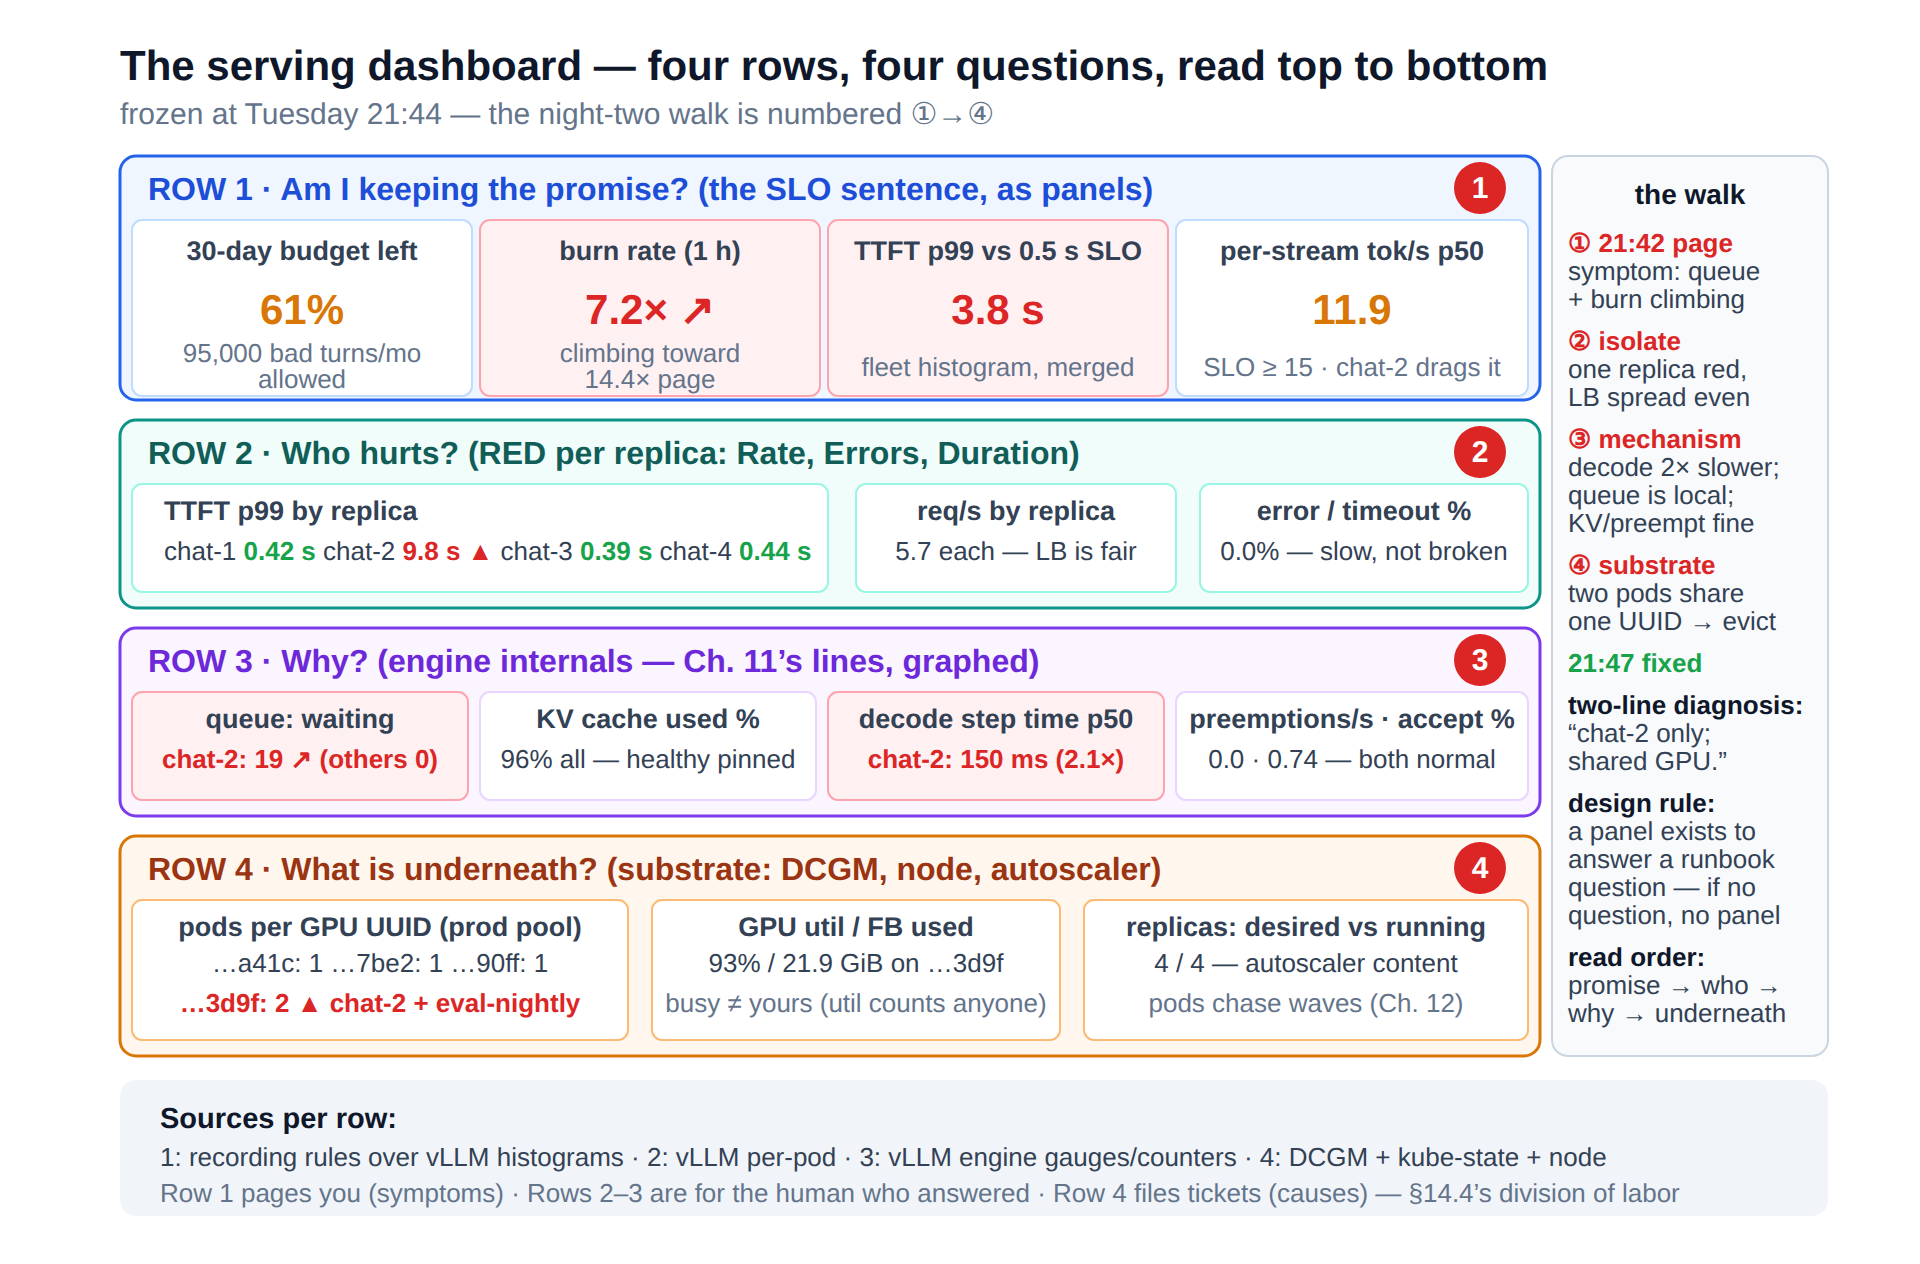
\includegraphics{figures/fig14-4_dashboard.png}}\\[3pt]
  \figcaption{그림 14-4  화요일 21시 44분에 멈춰 세운 네 행 서빙 대시보드. 1행은 “약속을 지키고 있는가?”에 답한다. SLO 문장을 예산, 소진율, 플릿 p99, 스트림별 속도 패널로 옮겼다. 2행은 “누가 고통받는가?”에 답하며 레플리카별 RED를 보여 준다. 3행은 “왜 그런가?”에 답하며 대기열, KV, 디코드 속도, 선점 등 엔진 내부를 보여 준다. 4행은 “그 아래에는 무엇이 있는가?”에 답하며 UUID별 DCGM, GPU당 파드, 오토스케일러 태세를 보여 준다. 둘째 날 밤의 조사 순서는 ①→④로 표시했다.}
\end{tbbfigure}

\textbf{1행은 “약속을 지키고 있는가?”에만 답한다.} 패널은 SLO 문장의 각 항목을 그대로 옮긴다. 30일 오류 예산 게이지에는 61\%가 남아 있다. 7장에서 제품 관리자와의 논쟁을 끝내 줄 것이라고 약속한 바로 그 그래프다. 14.4× 호출 임계선을 그린 소진율, 올바른 방식으로 계산한 플릿 TTFT p99(질의 2를 기록 규칙으로 만든 것), 15 이상이라는 조항과 비교한 스트림별 tokens/s p50도 있다. §14.4의 용어로 이곳의 모든 값은 사용자가 볼 수 있는 약속 위반, 즉 \textit{증상}이다. 따라서 1행만 사람을 깨운다. \textbf{2행은 “누가 고통받는가?”에 답한다.} 같은 RED 신호를 레플리카별, 경로별로 나눈다. 모든 용량 사고에서 첫 진단 갈림길은 \textit{모두가 느린가?}와 \textit{일부만 느린가?}이기 때문이다. 전자는 무릎점, 물결, 폭풍 같은 수요 문제이고 후자는 이번 화요일과 같은 머신 문제다. 파드별 TTFT p99와 로드 밸런서의 요청률을 나란히 둔 패널이 한눈에 갈림길을 결정한다. 트래픽은 네 곳에 공평하게 나뉘지만 고통은 한 곳에 불공평하게 몰린다. \textbf{3행은 엔진의 언어로 “왜 그런가?”에 답한다.} 11장의 선들이 마침내 그래프가 된다. 파드별 \code{num\_requests\_waiting}은 선행 지표이자 11장에서 “바로 그 경보”라고 부른 선이다. KV 캐시 점유율은 플릿 전체에서 높게 고정되어 정상이다. 새벽 2시의 뇌가 같은 오해를 되풀이하지 않도록 패널에 정상이라고 주석을 달아 둔다. 디코드 단계 속도는 원인을 구분한다. 대기열이 생기면서 디코드도 느리면 머신 자체가 느려진 것이고, 디코드는 정상인데 대기열이 생기면 수요가 좌석을 추월한 것이다. 선점률과 초안 수락률은 각각 풀 압력과 추측의 건전성을 보여 준다. 9장에서 대기열 시간과 계산 시간을 별도 카운터로 받아 “14주차 대시보드 설계의 절반이 이미 끝났다”고 약속했다. 3행은 분류기에서 그 약속을 지키고 LLM으로 일반화한다. \textbf{4행은 “그 아래에는 무엇이 있는가?”에 답한다.} UUID별 DCGM을 GPU당 파드와 조인한다. 프로덕션의 모든 행이 1이어야 하는 표에서 화요일의 결정적 증거가 드러난다. 프레임버퍼, Xid, 노드 활력 징후, 오토스케일러가 원하는 파드 수와 실행 중인 파드 수도 보여 준다. 파드는 물결을 뒤쫓는다. 파드가 \textit{뒤쫓지 않는} 물결은 별도의 사고 유형이며, 12장의 안정화 구간이 평탄한 지연으로 드러난다.

이제 이 설계가 어떻게 값을 치르는지 보자. §12.4에서 예고한 사고를 이 네 행으로 실시간 해결한다. 13장 마지막 상자에서 \textit{라이브로} 보여 주겠다고 약속한 시연이다. \textbf{21시 42분, 호출}(①): chat-2에서 QueueSustained가 발생한다. 호출 본문에는 런북 링크 R2가 있고 대시보드는 이미 경보 레이블로 필터링되어 있다. 1행에서 소진율이 7.2×로 계속 오르고 플릿 p99가 3.8 s임을 확인한다. 30초면 호출이 진짜임을 알 수 있고 질의는 하나도 입력하지 않는다. \textbf{②, 2행의 갈림길:} 레플리카별 TTFT p99는 0.42 / 9.8 / 0.39 / 0.44다. 모두가 아니라 \textit{일부}만 느리다. 레플리카별 req/s는 모두 5.7이므로 로드 밸런서는 공정하며 고통의 원인은 chat-2 자체에 있다. 모두와 일부를 가른 순간 “무릎점인가? 폭풍인가? 배포 때문인가?”라는 불안의 나무 전체가 사라진다. 배포는 없었고 수요 문제도 아니다. \textbf{③, 3행의 메커니즘:} chat-2의 대기열은 19지만 KV는 다른 파드와 같은 96\%이므로 풀 문제가 아니다. 선점도 늘지 않아 요동치는 상태가 아니다. 하지만 디코드 단계 p50은 플릿의 70에 비해 150 ms다. \textit{머신 자체}가 2.1× 느리다. 10장의 루프라인과 11장의 20 ms 하한을 떠올리면, 메모리 병목 루프의 경우 다른 무언가가 이 카드의 메모리 버스를 마시고 있다는 뜻이다. \textbf{④, 4행의 기반:} UUID당 파드 표에는 GPU …3d9f: 2(chat-2, eval-nightly-28471)라고 나온다. 이웃이 여기 있다. \code{kubectl delete job eval-nightly}를 실행하고, 노드의 오래된 시분할 ConfigMap을 조사하도록 격리 메모를 남긴다. 21시 50분이 되면 대기열이 비워지고 소진율은 1× 아래로 내려가 호출이 자동으로 해제된다. 사람이 들인 시간은 8분이고, 그중 입력에 쓴 시간은 2분이다. \textit{“chat-2만 문제, GPU 공유”}라는 두 줄 진단은 6장의 기념 문구가 염원에서 워크플로로 발전한 결과다. 행 자체가 두 줄을 작성한다. 2행이 첫 줄을, 4행이 둘째 줄을 쓴다.

재현 과정을 정직하게 만드는 세 가지 주석이 있다. 첫째, 21시 31분의 \textbf{원인 티켓}(GPU당 파드 = 2)은 호출보다 11분 먼저 범인을 지목했다. 둘째 날 밤이라면 사용자가 고통을 느끼기 전에 당직자가 Slack에서 읽을 수도 있었다. 그래도 호출 대신 티켓을 만드는 이유는 §14.4에서 설명한다. 원인은 셀 수 없이 많고 저렴하며 해가 없는 경우도 흔하다. 증상은 적고 비싸며 정의상 실제로 발생한 일이다. 약속 위반에 호출을 보내고 원인은 주석으로 붙인다. 둘째, 대시보드에 \textit{없었던} 것을 살펴보자. “시분할 충돌”이라는 패널은 없었다. 아무도 이 실패를 예측하지 못했지만 네 행은 답을 찾아냈다. 각 행이 알려진 실패를 열거하는 대신 \textit{질문}에 답하도록 설계되었기 때문이다. 이것이 관측 가능성의 역할이다. Aaron은 훈련에서만 본 잡음을 알아보았다. 셋째, 수정은 \textbf{기록}을 남겼다. 13장의 런북이 있는 레지스트리 항목에 사고 메모를 등록했고, 이제 WATCH 단계에는 “/metrics를 curl로 받아 눈을 가늘게 뜨고 본다” 대신 “대시보드 1\textasciitilde{}2행”이라고 적혀 있다. §14.4의 사후 분석 조치로 새 경보도 하나 추가했다. 실습 문제였던 GPU당 파드 규칙이 플릿 정책이 되었고 패널 캡션 하나도 수정했다. 사고 후에도 바뀌지 않은 대시보드는 아무것도 배우지 못한 대시보드다. 사고가 계측을 개선하는 순환 덕분에 모니터링의 가치가 \textit{복리로} 쌓인다. 이 순환은 10장 실습에서 사고 검토자가 읽을 수 있도록 게이트 보고서를 저장하게 했을 때 조용히 시작되었다.

\begin{calloutbox}{tbbred}{tbbxFEF2F2}
{\normalsize\bfseries\color{tbbx991B1B}상자 14-1  서빙 대시보드의 일곱 가지 치명적 죄악}\par\vspace{3pt}
\begin{tbbitemize}
  \item \textbf{전광판을 차지한 평균값.} 치우친 분포 위에 평균을 제목처럼 내세우면 사례 14-A의 “40\% 상승, 사용자가 과장한다”라는 결론에 이른다. 언제나 백분위수나 히스토그램을 써야 한다. 평균은 누구도 설명하지 못한다.
  \item \textbf{백분위수의 평균.} 레플리카별 p99에 avg()를 적용하면 실제 9.08 s 대신 2.76 s가 나온다. 버킷을 합친 뒤(sum by le) 분위수를 구해야 한다. 압박 속에서 즉석 질의를 만들 때도 예외는 없다.
  \item \textbf{사용률을 여유 용량으로 해석하기.} GPU 사용률은 점유 듀티 사이클이다. 바쁨 ≠ 내 것 ≠ 효율적임이다. 사용률이 의미하는 척하는 정보는 포화 신호인 대기열, 선점, DRAM 활동에 담겨 있다.
  \item \textbf{그래프에 SLO 선이 없음.} 0.5 s 임계선을 그리지 않은 p99 패널은 새벽 2시의 기억력에 판단을 떠넘긴다. 약속을 측정하는 모든 패널에 그 약속을 선으로 그려라.
  \item \textbf{런북 없는 경보, 질문 없는 패널.} 모든 호출은 런북으로 연결되고, 모든 런북 단계는 특정 행을 지목하며, 모든 패널은 런북이 그 질문을 하기 때문에 존재해야 한다. 그 밖의 것은 장식일 뿐이다.
  \item \textbf{모든 것을 쌓은 벽.} 알파벳순 패널 마흔 개는 어떤 질문에도 답하지 못한다. 약속 → 누구 → 원인 → 기반의 순서로 배치한 네 행은 위에서 아래로 1분 안에 읽을 수 있다. 지표마다 패널 하나가 아니라 독자마다 대시보드 하나를 만든다.
  \item \textbf{버전 관리하지 않는 대시보드.} JSON을 저장소에 두고 코드처럼 검토해야 한다. 그렇지 않으면 파드가 한 번 다시 스케줄되는 순간 계기판이 기억을 잃는다. 모니터링판 금요일 배포 사고다.
\end{tbbitemize}
\end{calloutbox}

\begin{calloutbox}{tbbpurple}{tbbpurplefill}
{\normalsize\bfseries\color{tbbpurple}생각해 보기}\par\vspace{3pt}
\begin{tbbitemize}
  \item 2행이 없다고 가정하고 둘째 날 밤의 조사 과정을 재구성하라. 어떤 질문에 답하기가 어려워지고, 당직자는 어떤 순서로 확인하게 되며, 첫째 날 밤에 걸린 49분 가운데 얼마나 되돌아오는가? 이는 “어느 행을 없앨 것인가?”라는 채점 문제의 본뜻이다. 답은 취향이 아니라 논증이어야 한다.
  \item 플릿 p99 패널(질의 2)과 SLI 비율 패널(질의 4)은 서로 다른 결론을 낼 수 있다. p99는 0.5 s 이하인데 SLI 비율은 목표보다 낮은 5분 구간과, 그 반대인 구간을 각각 구성하라. 호출기와 연결된 1행에는 어느 값을 넣어야 하는가? §14.4가 비율을 선택하는 이유는 무엇인가?
  \item 팀원이 “비즈니스 — 가입자 수, 판매한 토큰 수, 분당 매출”이라는 다섯 번째 행을 원한다. 독자, 갱신 주기, 조치하는 사람을 고려해 \textit{이} 대시보드에 넣어야 한다는 주장과 넣지 말아야 한다는 주장을 모두 제시하라. 12장의 단위 경제성 선이 실제로 속해야 할 위치도 설명하라.
  \item GPU당 파드 패널에는 UUID 레이블이 붙은 DCGM과 장치 플러그인의 파드 매핑을 조인해야 했다. 클러스터의 DCGM 익스포터에 파드 레이블이 없다면 당직자가 21시 44분에 수행할 두 단계 수동 조인을 설계하고, 첫날 밤의 49분과 비교해 몇 분이 더 드는지 추정하라.
\end{tbbitemize}
\end{calloutbox}

\section{경보: Page, 소진율, 거짓 경보를 피하는 기술}

Dashboard가 기억이라면 \textbf{alert}는 주의력이다. 어느 시간이든 사람을 지금 당장 깨워야 한다고 대신 결정하는 장치다. 이 결정에도 serving path와 같은 수준의 엔지니어링 엄밀함이 필요하다. 역사상 가장 좋은 사례는 가장 가까운 pager에서 40만 km 떨어진 곳에서 일어났다. 1969년 7월 20일, 최초의 달 착륙을 위한 powered descent가 시작된 지 5분 뒤 guidance computer에 \textbf{1202}가 떴다. Capsule 안에서 아무도 외우지 않은 alarm code였다. 연료는 타고, 표면은 다가오는데 crew의 화면은 뜻을 알 수 없는 네 자리 숫자만 내놓았다. 30초도 지나지 않아 지상에서 GO라는 판단이 왔고, 근거는 \textbf{손으로 쓴 cheat sheet}였다. 3주 전 훈련 simulation에서 관제팀은 자매 alarm인 1201을 보고 당황해 abort를 선언했다. 나중에 \textit{잘못된 판단}으로 드러났고 simulation supervisor는 교훈을 뼈아프게 남겼다. Backroom의 24세 엔지니어 Jack Garman은 집에 돌아가 모든 program alarm code를 손으로 쓰고, 각각이 문제가 되는 조건을 옆에 적었다. Executive overflow 계열에 붙인 메모의 뜻은 이랬다. \textit{너무 자주 반복되지 않고 guidance가 계속 작동하면 GO.} 실제로 1202가 떴을 때 front room의 Steve Bales가 Garman의 판정을 전달했고 Armstrong은 하강을 계속했다. Alarm은 이후 세 번 더 울렸지만 아무 문제도 생기지 않았다. Computer가 overload 상태임을 알리면서도 \textit{설계대로 우선순위가 낮은 작업을 버리고} 있었기 때문이다. Margaret Hamilton의 priority executive는 4 KB RAM 위에서 제9장의 부하 차단 원칙을 실행하고 있었다.

이 이야기에는 이 절의 모든 규칙이 들어 있다. Alarm의 의미는 \textbf{미리 글로 정했다.} \textit{실패한 drill}에서 태어난 runbook이다. 실습의 두 번 깨뜨리기에는 반세기가 넘는 전통이 있는 셈이다. 판정은 \textbf{존재가 아니라 비율과 지속성}을 기준으로 했다. "너무 자주 반복되지 않는다"는 1969년판 \code{for: 5m}과 rate threshold다. 무엇이든 spike 한 번만으로 page를 울릴 일은 거의 없다. Alarm이 울린 system은 \textbf{설계대로 우아하게 성능을 낮추고 있었다.} 어떤 alarm은 설계가 \textit{제대로 작동함}을 나타낸다. KV cache가 높게 고정되어 있거나 executive가 task를 버리는 경우다. 이런 상태마다 page를 보내면 사람은 page를 무시하도록 훈련된다. 이 원칙을 어길 때 사람이 치르는 대가는 우주 비행 밖에서 실제 사망자 수로 나타난다. 지금껏 만들어진 가장 빽빽한 alarm 환경인 병원 telemetry 병동은 업계에 \textbf{경보 피로(alert fatigue)}라는 용어를 가르쳤다. Joint Commission의 2013년 sentinel-event alert는 3년 반 동안 alarm 관련 사고 98건, 그중 사망 사고 80건을 집계했다. 임상 alarm의 \textbf{85–99\%는 아무 조치도 필요하지 않다}는 연구도 인용했다. Beep에 빠진 간호사는 합리적으로 beep가 아무 의미도 없다고 학습하고, 그러다 어느 하나가 실제 의미를 갖는다. 엔지니어링으로 옮기면 잔인하면서도 명쾌하다. \textit{행동할 수 있고, 긴급하며, 실제인} 조건이 아닌 모든 alert는 팀이 정말 중요한 하나를 놓치도록 적극적으로 훈련한다. Page는 정보가 아니라 잠에서 깨라는 명령이다. 적게 발행해야 한다.

\subsection*{증상은 page로, 원인은 ticket으로}

"적게 발행하라"를 운영 규율로 만드는 것은 Rob Ewaschuk의 \textit{My Philosophy on Alerting}와 뒤이은 SRE 책이 정착시킨 두 단어짜리 routing 원칙이다. \textbf{증상은 page로, 원인은 ticket으로 보낸다.} \textit{증상}은 사용자가 볼 수 있는 약속 위반이다. SLI가 피를 흘리고, queue가 요청을 빠뜨리며, 바깥에서 문이 열리지 않는 상태다. \textit{원인}은 언젠가 증상을 만들 수 있는 조건이다. 새는 레플리카, 오래된 ConfigMap, GPU 하나에 올라간 pod 두 개가 예다. 이 규칙을 정당화하는 비대칭이 있다. 증상은 \textbf{적고, 정의상 실제이며, 완전하다.} 상상하지 못한 것을 포함해 사용자를 해치는 모든 실패는 결국 SLI에 나타나야 한다. 화요일의 time-slice 충돌은 alert rule을 작성한 뒤 생겨났지만 queue page가 잡아냈다. 반면 원인은 \textbf{무수하고, 저렴하며, 흔히 무해하다.} \textit{Dev} pool에서 pod 둘이 같은 GPU를 쓰는 일은 화요일에도 정상이다. §12.4가 그곳에서는 time-slicing을 정직하게 권했다. 원인마다 page를 울리면 새벽 3시의 무의미한 사건에 무감각해진 병원 병동 같은 rotation이 된다. 그래서 화요일의 GPU별 pod alert는 \textbf{ticket}을 만들었다. 21:31에 Slack에서 볼 수 있었고, \textit{증상이 관련성을 부여한 순간} 엄청난 가치를 발휘했지만 pager는 울리지 않았다. 그날 밤 유일한 page는 queue였다. 사용자가 이미 기다리고 있던 선행 증상이라 24분 늦게 울릴 burn-rate page라는 후행 증상을 앞섰다. 제3장의 memory.high처럼 벽 앞에 tripwire를 놓는 방식이다. 표 14-1이 지속 gauge 가운데 유일한 PAGE를 제11장에서 바로 이 역할을 맡긴 \code{num\_requests\_waiting}에 배정한 이유다.

\subsection*{SLO 문장 컴파일하기: 오류 예산과 소진율 계산}

제13장은 이 장에서 "느낌이 아니라 소진율에 따라 page가 울리게" 만들겠다고 약속했다. 이제 과정 SLO의 availability 조항을 처음부터 끝까지 compile해 보자. 11주 차 계약은 \textbf{TTFT p99 ≤ 500 ms}라고 말한다. 이는 \textit{turn의 99\% 이상이 0.5초 안에 첫 token을 받는다}는 문장과 같다. 비율로 다시 쓰면 \textbf{SLI}가 되고(터미널 기록 14-2의 query 4), 나머지 1\%는 \textbf{오류 예산}이 된다. 플릿은 한 달에 약 950만 turn, 즉 평균 답변 약 211 token으로 20억 token을 서빙하므로 이 약속은 \textbf{30일마다 나쁜 turn 약 95,000개}를 허용한다. 제7장이 시간 기준 99.9\%를 43분이라는 자원으로 표현한 것과 같다. 단위가 달라졌음에 주목하자. 요청 기준 budget은 분이 아니라 turn을 세므로 하루 주기의 traffic 파동에서도 의미가 유지된다. 새벽 3시의 나쁜 \textit{1분}은 거의 쓰지 않지만 21:30의 나쁜 1분은 큰 비용을 쓰며, 사용자 고통을 이렇게 가격화하는 것이 옳다. \textbf{소진율}은 소비 속도다. Burn = 나쁜 turn 비율 ÷ (1 − SLO)다. 1×로 소진하면 정확히 30일 만에 budget을 모두 쓴다. 손익분기 속도인 셈이다. 화요일 21:44에 chat-2가 도착 요청의 4분의 1을 빠뜨렸으므로 나쁜 비율은 약 24\%, burn은 약 24×였다. 한 달 budget을 30시간 만에 쓰는 속도다. 그림 14-5는 tank와 drain을 그린다.

\begin{tbbfigure}
  \adjustbox{max width=0.94\linewidth,max totalheight=0.46\textheight}{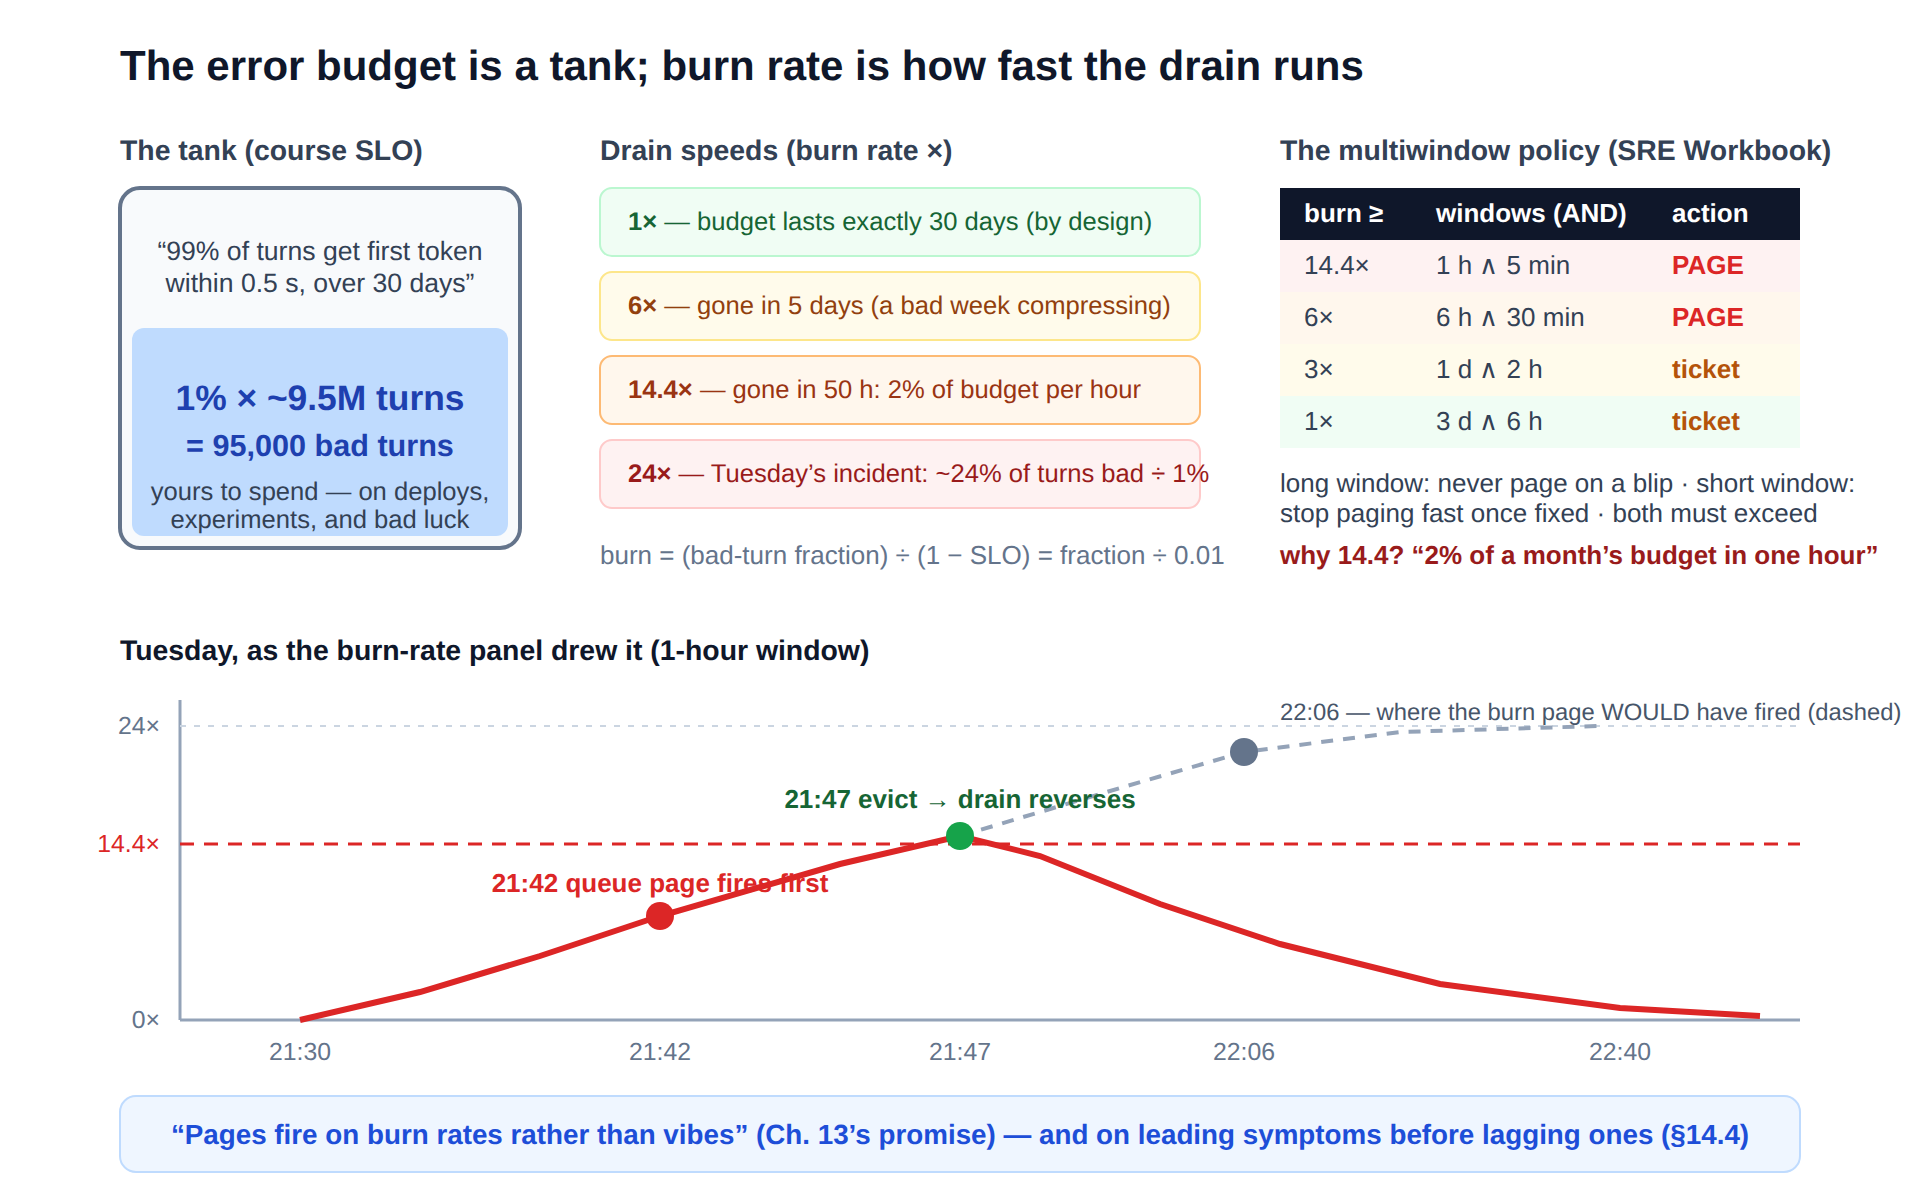
\includegraphics{figures/fig14-5_burnrate.png}}\\[3pt]
  \figcaption{그림 14-5  Budget tank(나쁜 turn 95,000개), 네 가지 drain 속도, 여러 window 정책, 1시간 burn panel에 그린 화요일의 모습. Queue page가 burn page보다 24분 먼저 울렸고, 점선은 완화하지 않았을 때 burn page가 울릴 시점인 22:06을 나타낸다.}
\end{tbbfigure}

Burn 경보는 window를 다루는 게임이다. 실습이 그대로 채택한 SRE Workbook의 표준 정책은 심각도마다 \textbf{window 두 개를 짝지어} 사용한다. Burn이 \textbf{1시간과 5분 모두에서 14.4× 이상}이면 page를 울린다. 이 속도는 한 시간마다 월간 budget의 2\%를 쓴다. \textbf{6시간과 30분에서 6×}면 page를 울린다. 6시간마다 5\%를 쓰는 속도로, 빠른 rule이 놓치는 느린 출혈을 잡는다. \textbf{하루 동안 3×}, \textbf{3일 동안 1×}면 낮에 처리할 trajectory 경고인 ticket을 만든다. 각 짝은 기질의 절충을 하나 담는다. \textbf{긴 window는 의심}이다. 깊이가 아무리 커도 90초짜리 blip은 1시간 평균을 14.4× 너머로 움직일 수 없어 page를 울리지 않는다. Apollo의 "너무 자주 반복되지 않는다"를 산술로 옮긴 것이다. \textbf{짧은 window는 용서}다. 사고가 끝나면 5분 평균이 즉시 내려가 page가 해제된다. 긴 window가 빠지는 동안 나머지 한 시간 내내 울리지 않는다. 의심의 정직한 비용은 latency다. 화요일의 24× burn에서 1시간 평균이 14.4×를 넘는 데 약 35분이 필요했다(24 × 35/60 = 14). 그래서 alert 목록은 burn에만 의존하지 않는다. Burn page는 \textbf{완전성 보장}이다. 이미 알든 새롭든 사용자가 볼 수 있는 모든 실패가 결국 이를 울린다. Queue page는 이 플릿이 실제로 겪는 실패의 \textbf{빠른 경로}다. Capacity 형태의 고통은 제7장의 knee와 제11장의 admission line처럼 queue에 먼저 나타난다. 빠른 경로는 허용하지만 증상에만 준다.

\begin{terminalbox}
\begin{Verbatim}[breaklines=true,breakanywhere=true,fontsize=\small,formatcom=\color{tbbtermfg},codes=\tbbcodeactive]
# monitoring/rules-alerts.yaml (excerpt) -- the roster's teeth
- alert: SLOBurnFast                              # completeness guarantee
  expr: >
    (1 - job:slo_ttft_good:ratio_rate1h) / 0.01 > 14.4
    and (1 - job:slo_ttft_good:ratio_rate5m) / 0.01 > 14.4
  labels: { severity: page }
  annotations: { runbook: runbooks/R1-slo-burn.md }

- alert: QueueSustained                           # fast path (symptom)
  expr: avg_over_time(vllm:num_requests_waiting[5m]) > 8
  for: 5m
  labels: { severity: page }
  annotations: { runbook: runbooks/R2-queue.md, dashboard: row 3 }

- alert: DuplicatePodsOnProdGPU                   # cause (tuesday's vaccine)
  expr: count by (UUID) (DCGM_FI_DEV_GPU_UTIL{pool="prod"}) > 1
  for: 2m
  labels: { severity: ticket }

- alert: Watchdog                                 # dead man's switch
  expr: vector(1)                                 # fires ALWAYS, on purpose
  labels: { severity: heartbeat }

# alertmanager.yaml (excerpt) -- routing, grouping, silence
route:
  group_by: [alertname, model]      # one incident = one page, not 40
  routes:
  - match: { severity: page }    receiver: oncall-phone
  - match: { severity: ticket }  receiver: slack-serving-alerts
  - match: { severity: heartbeat } receiver: deadman-external
$ amtool silence add alertname=QueueSustained --duration=2h \
    --comment "drill A in progress (lab 14)"      # planned breakage, quiet
\end{Verbatim}
\end{terminalbox}
\figcaption{터미널 기록 14-4  Alert는 심각도를 가진 query이고 routing은 정책이다. 형태에 주목하자. Burn 짝은 recording rule을 읽고, queue page에는 지속 조건(for: 5m)이 필요하며, 원인 rule은 ticket을 만든다. Watchdog는 영원히 울리므로 heartbeat를 기다리는 외부 receiver가 감지한 \textbf{침묵}은 monitoring stack 자체가 멈췄다는 뜻이다. 감시자는 누가 감시하는가? 사람이 쓰러지면 놓이는 switch가 감시한다.}

\begin{tbbtablewrap}
  \begin{tabular}{@{}>{\raggedright\arraybackslash}m{\dimexpr 0.2500\tbltextwidth-2\tabcolsep\relax} >{\raggedright\arraybackslash}m{\dimexpr 0.3085\tbltextwidth-2\tabcolsep\relax} >{\raggedright\arraybackslash}m{\dimexpr 0.1223\tbltextwidth-2\tabcolsep\relax} >{\raggedright\arraybackslash}m{\dimexpr 0.3191\tbltextwidth-2\tabcolsep\relax}@{}}
  \arrayrulecolor{tbbnavy}\specialrule{1pt}{0pt}{0pt}
  \rowcolor{tbbtablehead}{\centering \bfseries\color{tbbnavy}경보} & {\centering \bfseries\color{tbbnavy}조건(개요)} & {\centering \bfseries\color{tbbnavy}심각도} & {\centering \bfseries\color{tbbnavy}존재 이유 · 계보} \\
  \arrayrulecolor{tbbnavy}\specialrule{0.7pt}{0pt}{2pt}
  {\textbf{SLOBurnFast}} & {1시간 ∧ 5분 동안 burn ≥ 14.4×} & {PAGE} & {약속이 빠르게 무너짐. 상상하지 못한 실패도 잡는다(제7장 → 여기).} \\
  \arrayrulecolor{tbbtableborder}\hline
  {\textbf{SLOBurnSlow}} & {하루 동안 burn ≥ 3×(그리고 3일간 1×)} & {ticket} & {궤적 경고. 낮에 의도적으로 budget을 사용한다.} \\
  \arrayrulecolor{tbbtableborder}\hline
  {\textbf{QueueSustained}} & {어느 pod든 5분 동안 waiting > 8} & {PAGE} & {빠른 경로. Capacity 고통은 queue에 먼저 온다(제11장의 alarm line).} \\
  \arrayrulecolor{tbbtableborder}\hline
  {\textbf{EndpointsEmpty}} & {chat Service의 ready address = 0} & {PAGE} & {Routing 대상이 없으면 지금 모든 사용자가 제6장의 503을 본다.} \\
  \arrayrulecolor{tbbtableborder}\hline
  {\textbf{ProbeFail}} & {어느 probe든 probe\_success = 0이 3회 연속} & {PAGE} & {밖에서 문이 열리지 않음. 플릿이 볼 수 없는 계층이다(제6장).} \\
  \arrayrulecolor{tbbtableborder}\hline
  {\textbf{PreemptionSurge}} & {10분 동안 rate(preemptions) > 0.5/s} & {ticket} & {KV pool thrashing. Prompt-length drift가 도착할 때가 많다(§14.5).} \\
  \arrayrulecolor{tbbtableborder}\hline
  {\textbf{RestartsOOM}} & {Δrestarts ≥ 3/h 또는 OOMKilled 발견} & {ticket → 플릿 전체면 page} & {Self-healing이 leak을 감춘다(제5장 목록, 제3장 exit 137).} \\
  \arrayrulecolor{tbbtableborder}\hline
  {\textbf{DuplicatePodsOnProdGPU}} & {2분 동안 prod UUID별 pod > 1} & {ticket} & {화요일을 막는 백신. 원인이므로 깨우지 않고 주석을 남긴다.} \\
  \arrayrulecolor{tbbtableborder}\hline
  {\textbf{Watchdog}} & {vector(1), 항상 firing} & {heartbeat} & {Dead man’s switch. Cluster 밖 receiver가 그 침묵을 page로 보낸다.} \\
  \arrayrulecolor{tbbnavy}\specialrule{1pt}{2pt}{0pt}
  \end{tabular}\par
  \figcaption{표 14-2  경보 목록. Page 네 개는 모두 증상이고 runbook을 갖췄다. Ticket 네 개는 모두 원인이며 heartbeat가 하나 있다. 수백 개가 울리는 병동과 비교해 보자. 자기 pager를 믿는 rotation이 이 표의 결과물이다.}
\end{tbbtablewrap}

\subsection*{Synthetic probe: 거부할 수 있는 모든 계층의 바깥에 서기}

앞의 모든 장치는 플릿의 벽 안에서 플릿을 바라본다. 제6장은 그 시야가 얼마나 많이 놓치는지를 실습 하나로 증명했다. LB가 구현되지 않은 path를 health check하고, TLS가 만료되며, perimeter timeout이 자기 것보다 짧은 실패에서는 사용자가 503을 보는데 kubectl은 결백하다고 말한다. 증거가 \textit{cluster 바깥} console에 있기 때문이다. 모니터링의 답은 \textbf{synthetic probe}이며, 세 가지를 설계하라고 했던 제6장 연습문제의 공식 해답이 여기에 있다. 첫째는 \textbf{문}이다. Blackbox exporter가 public gateway URL에 30초마다 HTTPS \code{GET /\allowbreak v1/\allowbreak models}를 보낸다. DNS, TLS, LB target health, routing을 모두 거치며, \textit{LB 바깥에서 실행하지 않으면} 아무것도 검증하지 못한다. 검사 대상과 운명을 공유하는 probe는 증인이 아니라 거울이다. 매우 신중한 팀은 두 번째 region에서 실행한다. 둘째는 \textbf{답변}이다. 1분마다 10초 timeout으로 token 하나짜리 completion을 요청한다. Admission과 engine을 포함한 전체 경로를 거치며 문 probe가 그대로 통과하는 504/hang 부류를 잡는다. 셋째는 \textbf{stream}이다. 5분마다 짧은 streaming completion을 실행해 2초 안에 첫 token을 받고 마지막 chunk가 온전해야 한다. 제6장의 표 6-3이 답변 중간의 침묵 원인으로 지목한 \textit{idle-timeout} 계층 바깥에 서는 stream-cut detector다. Probe 세 개가 서로 다른 세 계층을 맡고 각각 책임을 물을 계층 바깥에 선다. \code{probe\_success}가 3회 연속 실패하면 page를 울린다. 한 번의 존재만으로 울리면 모든 network 재채기마다 page가 온다. Garman의 원칙이 다시 등장한다. 이들은 과정에서 가장 오래된 관측 가능성의 빈틈을 함께 닫는다. 사례 14-A의 uptime checker가 밤새 초록색이었던 이유는 \textit{첫 번째 probe만 있었기} 때문이다. 문이 살아 있다는 사실만 알렸고 뒤의 queue에 대해서는 아무 말도 하지 않았다. Synthetic은 과정에서 처음 LB target-health console로 보냈을 때의 약속을 완성한다. \textbf{관측 가능성은 거부할 수 있는 모든 계층을, 그 계층이 조작할 수 없는 시점에서 포괄해야 한다.}

\subsection*{사람이 맡는 절반: On-call, runbook, postmortem과 숫자의 가치}

Page는 사람에게 도착하며, 그 사람 주위의 장치도 PromQL만큼 세심하게 설계해야 한다. \textbf{On-call rotation}은 교대로 pager를 들고 명시적인 계약을 따른다. 몇 분 안에 응답하고, 부담 없이 escalate하며, 인수인계를 글로 남긴다. 표 14-2가 매일 밤이 아니라 한 달에 한 번쯤 page를 울리기 때문에 지속 가능한 구조다. \textbf{Page에는 runbook이 붙는다.} 제13장의 template에 이제 이가 생겼다. 증상 → 답을 주는 dashboard 행 → 되돌리기 쉬운 순서로 나열한 안전한 완화책 → escalation 연락처가 이어진다. 제13장에서는 \code{/\allowbreak metrics}와 script만 가리킬 수 있었던 runbook의 WATCH 단계가 이제 \textit{"1–2행, burn과 레플리카별 지표"}라고 적힌다. 해결 뒤에는 항공 분야와 John Allspaw의 노력을 통해 업계가 받아들인 \textbf{비난 없는 postmortem}이 이어진다. Blameless는 예의가 아니라 지식의 문제다. 개인은 일정한 비율로 실수하고 system이 그 가격을 정한다는 제13장의 논증처럼, 사람 이름으로 끝난 postmortem은 아무것도 배우지 못하지만 \textit{작동 원리}로 끝나면 action item이 생긴다. 화요일 사고에서는 하루 안에 세 가지를 기록했다. GPU별 pod rule을 실습 문제에서 플릿 정책으로 승격해 원인 alert답게 ticket으로 만들고, 오래된 time-slice ConfigMap에 owner와 CI expiry check를 부여했으며, dashboard caption 하나를 "busy ≠ yours"로 고쳤다. 보고서 자체는 v9-int4의 \textbf{registry 항목에 연결했다.} 제10장 실습이 언젠가 사고 검토자가 저장된 gate report를 읽을 것이라 했고, 바로 이 사람이 파일을 닫는다. 사고 → 계측이라는 순환이 모니터링에 \textit{복리}를 만든다. 불이 날 때마다 smoke detector 하나가 남는다.

장치 전체를 평가하는 숫자는 둘이며 몇 주 전부터 이 책이 열어 둔 장부를 닫는다. \textbf{MTTD}는 mean time to detect, 즉 사고 시작부터 사람이 알 때까지이고, \textbf{MTTR}은 mean time to restore, 즉 사고 시작부터 사용자가 정상 상태를 되찾을 때까지다. 그림 14-1의 36+49와 12+8 막대가 이를 보여 준다. MTTR은 DORA의 네 번째 key이며 제13장에서 나머지 셋의 가격을 계산했다. 과정의 배포 이야기는 네 key를 추정이 아니라 계측한 상태로 끝난다. 이 분포는 \textit{설계 입력}이기도 하다. 제13장 논술은 blue/green warm standby 시간을 어떤 data로 조정할지 물었다. 이제 답이 dashboard에 있다. 배포 형태 regression의 MTTD가 12분이면 비용이 2배인 warm standby를 한 시간 유지해도 약 20분 이후에는 얻는 것이 없으므로 window를 줄일 수 있다. 반대로 support 전화로 36분 뒤에야 감지하는 플릿은 예전 color를 일찍 없앨 수 없다. 제7장이 논술로 냈던 새벽 2시 상황, 즉 \textit{SLO를 위반했고 demo까지 6일 남았을 때 어느 조항을 적용할 것인가?}도 마침내 읽기 문제가 된다. 1행은 budget이 61\%이고 burn이 증가함을 보여 주며, 7주 차 결과물인 SLO 문서는 미리 합의한 완화와 owner를 밝힌다. 결정은 논술이 약속한 형태, 즉 논쟁이 아니라 산술과 서명으로 내려진다. 마지막 원장 항목도 확정하자. Prometheus, Grafana, Alertmanager, exporter, 50 GiB TSDB로 이루어진 monitoring stack은 cluster의 남는 CPU를 이용해 한 달 약 \textbf{\$23}가 든다. 합계는 \$877 + \$23 = \textbf{정확히 상한인 \$900}다. 과정 청구서의 마지막 항목은 다른 모든 항목을 감시하고, 그림 14-1 caption이 이미 비용 대비 효과를 계산했다. 이 stack은 첫 화요일에 한 달 값을 모두 갚았다.

\begin{calloutbox}{tbbpurple}{tbbpurplefill}
{\normalsize\bfseries\color{tbbpurple}생각해 보기}\par\vspace{3pt}
\begin{tbbitemize}
  \item Garman의 원칙은 “너무 자주 반복되지 않으면 GO”였다. 이 절에서 “너무 자주”를 표현하는 세 가지 서로 다른 장치(for:, avg\_over\_time, 짝지은 window)를 alert-rule 문법으로 옮기자. 각 장치는 어떤 실패 부류 때문에 page가 울리는 일을 막는가?
  \item “Queue depth는 원인이고 오직 SLI만 증상이다”라고 주장하는 엄격한 증상 우선주의자에게 QueueSustained page를 변호하자. 그 입장은 어느 지점에서 사용자에게 비용을 떠넘기는가? 빠른 경로가 정직하려면 queue threshold가 어떤 성질을 가져야 하는가? 힌트: SLI가 울리지 않을 때도 이 threshold가 울릴 수 있는가? 12주 차 autoscaler가 seat 수를 바꾸면 이 결합에는 어떤 유지보수가 필요한가?
  \item 화요일 사고의 inhibition rule을 설계하자. Chat-2에서 QueueSustained가 page를 울리는 동안 Alertmanager가 어떤 ticket을 억제해야 하며, 어떤 것은 절대 억제해서는 안 되는가? Watchdog 억제가 용납할 수 없는 configuration인 이유는 무엇인가?
  \item Dead man’s switch는 monitoring이 침묵하면 cluster \textbf{바깥} receiver를 통해 page를 울린다. Receiver가 (a) Slack webhook, (b) 만료된 card로 결제하는 phone service, (c) 같은 cloud region에서 hosting되는 경우에도 말없이 실패하는 것은 무엇인가? Probe와 heartbeat가 모두 지켜야 하는 shared fate의 일반 원칙을 도출하자.
\end{tbbitemize}
\end{calloutbox}

\section{드리프트: 절대 Page를 울리지 않는 실패}

지금까지 이 장에서는 \textit{시작점}이 있는 실패를 추적했다. 무언가 깨지는 순간이 있고 산술이 붙잡을 수 있는 window가 있었다. 하지만 registry가 몇 주 전 digest \code{a17b…}에서 model을 얼린 뒤에도, 어느 digest도 고정할 수 없는 input 하나가 남는다. 바로 세상이다. 사용자의 집단, 언어, 계절, 의도가 바뀌고, 뉴스는 존재하는 질문 자체를 바꾸며, 자기 성공도 찾아오는 사람을 바꾼다. 제12장 논술의 LMS integration처럼 학기 중간에 학생 1만 명이 플릿에 들어올 수 있다. Model은 고정된 어느 순간의 weights로 이 모든 변화를 맞는다. \textbf{Model은 바뀌지 않지만 세상은 바뀐다.} 둘 사이의 간격은 강줄기가 움직이듯 넓어진다. 절벽도 시작점도 alarm도 없다. 제13장은 blind spot을 정확히 이름 붙였다. \textbf{Canary는 경사면이 아니라 절벽을 잡는다.} 경사면은 여러 \textit{주} 동안 쌓은 production data로 만든 도구의 몫이라고 약속했다. 그 도구가 \textbf{drift detection}이다. 강의계획서가 이를 dashboard와 alarm 옆에 둔 것은 옳다. 아무것도 beep하지 않는 시간 규모에 기억과 주의력이라는 pattern을 적용하기 때문이다.

분류 체계는 대응할 때 가치를 발휘하므로 세 질문으로 익히자. \textbf{Data drift}(covariate shift)는 \textit{input} 분포 P(x)가 움직였는지를 묻는다. Prompt가 길어지고 한국어 비중이 두 배가 되며 새로운 주제 cluster가 나타난 경우다. 3B chat model에게 긴 prompt가 분포 밖 입력인 것은 아니므로 새 조합에서도 model 자체는 완벽히 유능할 수 있다. 보통 먼저 깨지는 것은 \textit{서빙 산술}과 \textit{평가 범위}다. §11의 prefill/KV budget은 이제 맞지 않는 input census를 기준으로 정했고, gate의 eval set은 예전 세상에서 표본을 뽑았기 때문이다. \textbf{Concept drift}는 같은 input에서 \textit{올바른 답} P(y|x)가 달라졌는지를 묻는다. "대통령은 누구인가?", "도서관 이용료는 얼마인가?"처럼 ground truth에 날짜가 붙는 질문이 예다. 어떤 serving metric도 concept drift를 볼 수 없다. Model은 유창하고 자신 있게 오래된 답을 내놓는다. 오직 지금 세상으로 새로 평가해야 잡을 수 있으며 대응 사다리의 둘째 칸이 존재하는 이유다. \textbf{Prior shift}는 \textit{과제의 구성} P(y)가 움직였는지를 묻는다. 시험 기간이 되면 일반 assistant가 proof checker가 되고, answer length 211과 refusal 0.8\% 같은 guardrail baseline이 조용히 중심을 옮긴다. 9월에 맞춘 threshold는 12월에 거짓 경보를 낸다. Drift detection은 \textit{다른} monitor를 정직하게 유지하는 장치이기도 하다. LLM에서는 세 부류를 잇는 결론이 하나 더 있다. \textbf{Eval set 자체도 drift한다.} 영원히 94.2\%를 기록하는 gate는 자기가 태어난 날의 세상을 측정한다. 성숙한 팀은 분기마다 production에서 eval slice를 다시 뽑고 baseline을 새로 잡으며, 그 diff 자체를 drift report로 남긴다.

\begin{tbbfigure}
  \adjustbox{max width=0.94\linewidth,max totalheight=0.46\textheight}{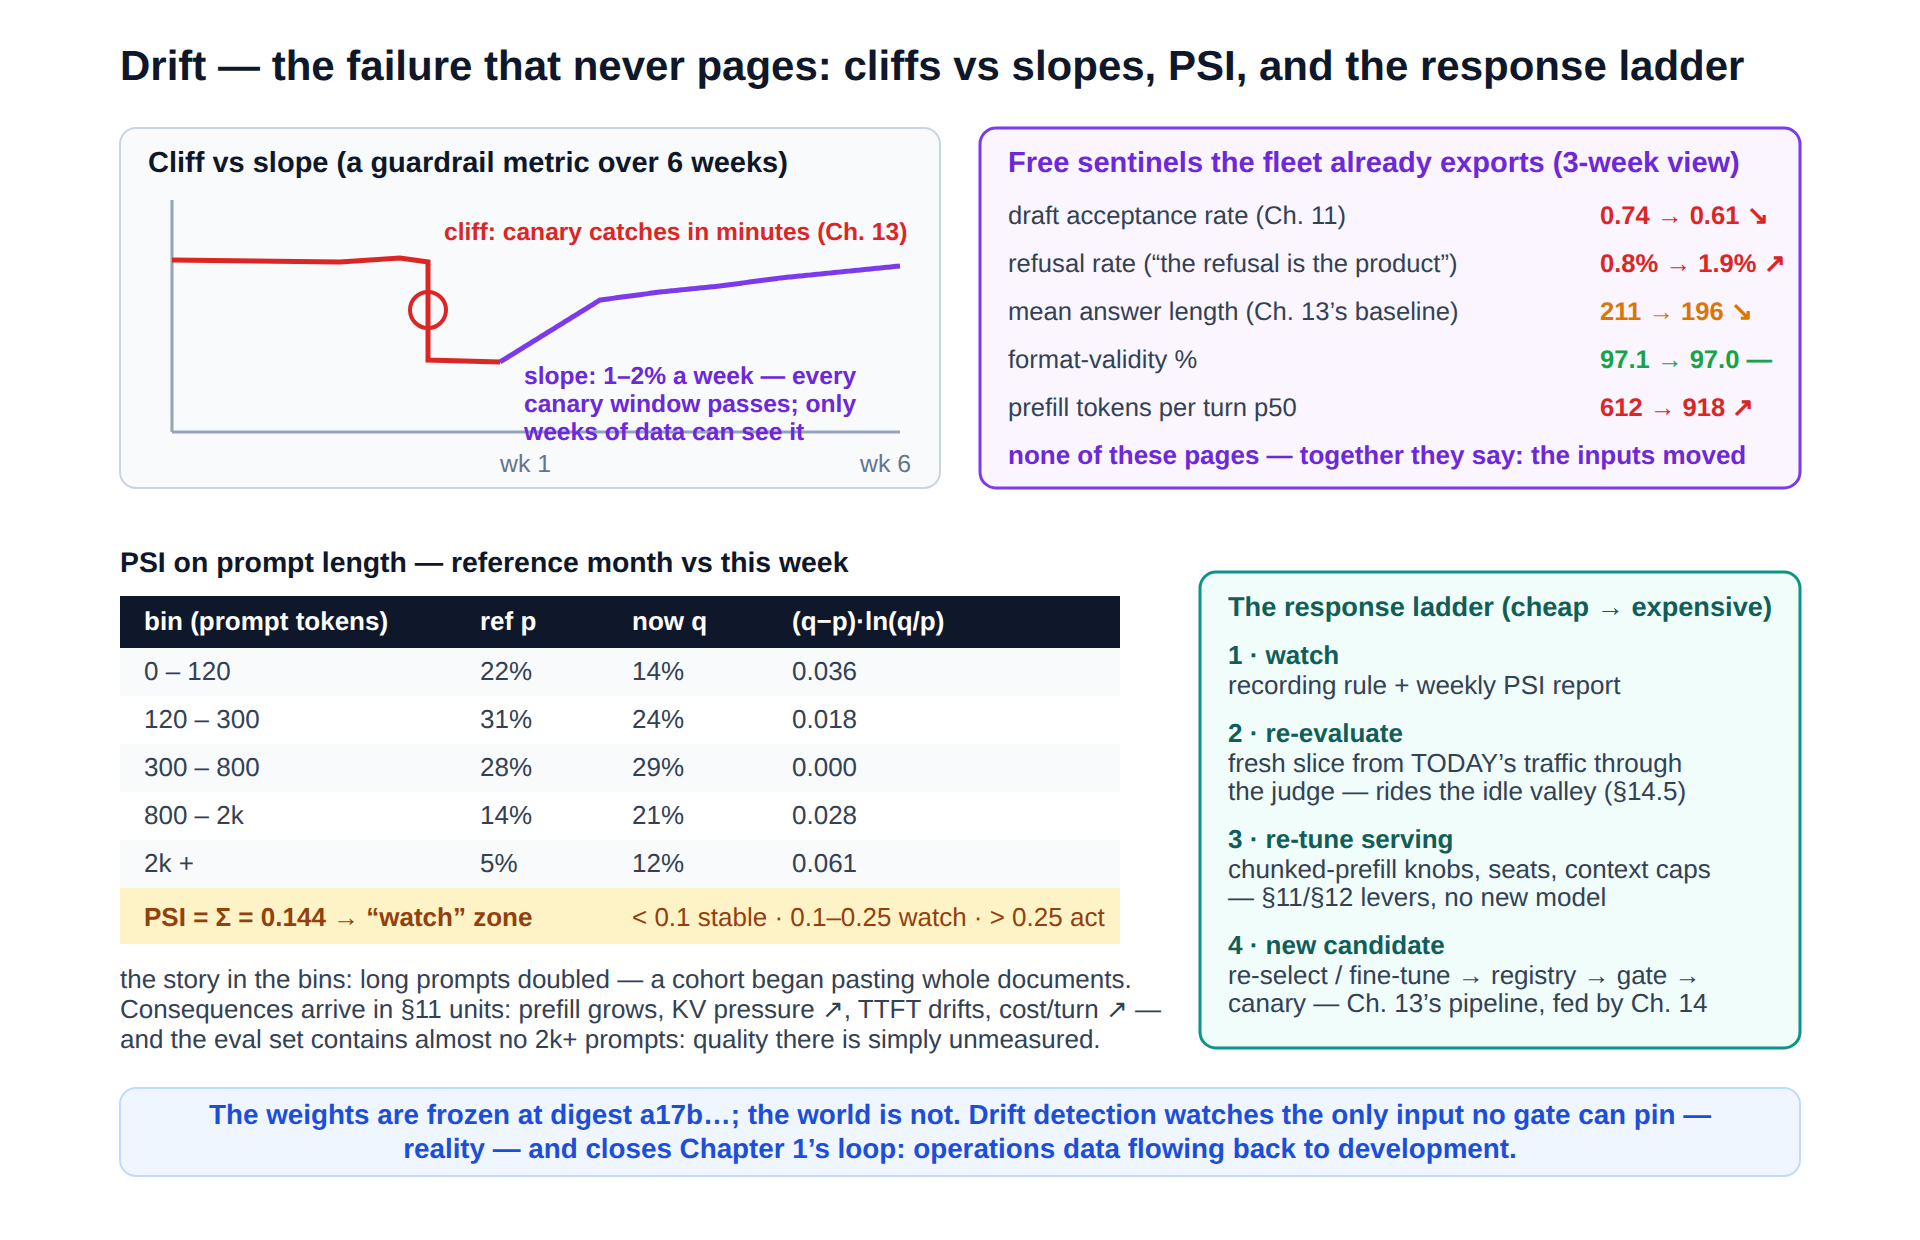
\includegraphics{figures/fig14-6_drift.png}}\\[3pt]
  \figcaption{그림 14-6  드리프트 계측. 왼쪽 위는 canary가 잡는 절벽과 여러 주가 지나야 보이는 경사면, 오른쪽 위는 플릿이 이미 내보내며 함께 움직이는 sentinel metric이다. 왼쪽 아래는 prompt length의 PSI를 손으로 계산한 결과인 0.144, 관찰 구간이다. 오른쪽 아래는 저렴한 대응에서 비싼 대응으로 올라가는 사다리다. 넷째 칸은 제13장의 pipeline으로 이어져 제1장의 순환 고리를 닫는다.}
\end{tbbfigure}

\subsection*{이미 내보내는 Sentinel과 손으로 계산할 수 있는 숫자 하나}

새로 만들기 전에 그림 14-6 오른쪽 위 panel부터 읽자. 11주 차부터 플릿이 내보낸 다섯 선은 어느 것도 page를 울리지 않지만 \textit{함께} 움직여 input이 변했음을 말한다. 3주 동안 0.74에서 0.61로 내려간 \textbf{draft acceptance rate}는 제11장의 열린 질문, 즉 \textit{speculative decoding의 조용한 실패를 어느 dashboard 선이 감지하는가?}에 대한 답이다. Acceptance는 작은 model이 실제 traffic을 얼마나 잘 예측하는지 실시간으로 추정하므로 무료로 상시 작동하는 분포 온도계가 된다. Input이 두 model 모두에게 편안한 영역에서 벗어나면 draft가 먼저 틀리고, speedup이 1×로 줄며, 선이 내려간다. 품질 비용보다 TPOT 비용이 먼저 오는 조기 경보 순서를 공짜로 얻는다. \textbf{Refusal rate}는 0.8\%에서 1.9\%로 서서히 오른다. Refusal 자체가 제품이지만, 그 비중이 \textit{늘면} 예전에 서빙하던 사람을 거부하거나 사람들의 구성이 달라진 것이다. \textbf{평균 answer length}는 제13장의 211-token baseline에서 새 중심으로 이동한다. \textbf{Format validity}는 평평하다. Input drift가 보이는 동안 capability drift를 배제하는 유용한 \textit{음성} sentinel이다. 마지막으로 \textbf{prefill token p50}이 612에서 918로 올라 다섯 선 가운데 가장 크게 외친다. §11의 결과도 즉시 나타난다. 긴 prompt는 admission마다 KV를 더 쓰고 preemption을 늘린다. 표 14-2의 PreemptionSurge ticket은 drift가 capacity plane을 통해 자신을 알리는 경우가 많다. 순전히 산술적인 이유로 TTFT가 SLO 선을 향한다. Sentinel은 저렴한 상관관계이지 증명이 아니다. 여러 선이 함께 움직이면 실제 분포 검사로 넘어간다.

업계에서 널리 쓰는 도구는 \textbf{Population Stability Index}다. 냅킨 위에서도 계산할 수 있어 vendor dashboard가 보여 줄 때 직접 \textit{감사}할 수 있다는 장점이 있다. \textbf{Reference window}, 즉 마지막 gate 실행 전후 한 달로 feature를 bin으로 나눈다. 이 기간은 eval set이 믿는 세상이다. 이번 주의 bin별 비중을 측정한 뒤 PSI = Σ (qᵢ − pᵢ) · ln(qᵢ/pᵢ)를 계산한다. Bin이 늘거나 줄면 각 항은 양수가 되며 상대 변화에 절대 이동량으로 가중치를 준다. 그림 14-6의 표는 prompt length에 적용했다. 2k+ bin이 5\%에서 12\%로 두 배 넘게 늘어 혼자 0.061을 기여하고, 합계는 \textbf{PSI = 0.144}다. 신용 평가 분야가 대출 신청자의 drift를 수십 년 동안 추적하며 물려준 관례적 구간(< 0.1 안정, 0.1–0.25 관찰, > 0.25 행동)에서 관찰에 해당한다. PSI를 정직하게 지키는 규율은 둘이다. 먼저 \textit{reference} quantile을 이용해 같은 질량의 bin을 만든다. 예전 세상에 질량이 있던 모든 곳에서 검사가 힘을 갖게 된다. 그리고 length, language, route, hour-of-day처럼 feature마다 별도로 실행한다. 조용한 합계가 반대 방향으로 drift하는 두 feature를 숨길 수 있기 때문이다. 손으로 bin을 나누기 어려운 의미에는 같은 방법을 \textbf{embedding}에 적용한다. 이번 주 prompt-embedding centroid와 reference centroid의 평균 cosine distance를 밤마다 계산하고, reference vector를 eval set 옆 registry에 저장한다. Model뿐 아니라 \textit{측정자}의 lineage도 남긴다. 통계적 엄밀함이 더 필요하면 Kolmogorov–Smirnov test가 bin 대신 CDF 사이의 supremum을 사용한다. p-value 보정은 더 좋지만 bin별 이야기를 해석하기는 어렵다. 이 과정이 PSI를 가르치는 이유는 "어느 사용자 집단이 document를 붙여 넣기 시작했다" 같은 \textit{bin 속 이야기}가 엔지니어가 실제로 행동할 수 있는 부분이기 때문이다.

\subsection*{대응 사다리와 판정 비용을 내는 사람}

대응을 정하지 않은 detection은 취미에 불과하다. 그래서 실습의 drift job은 모든 report를 그림 14-6 사다리의 어느 칸에서 끝낸다. \textbf{첫째 칸, 관찰}은 PSI가 관찰 구간에 있고 sentinel이 조용할 때다. 주석을 남기고 매주 실행하되 아무것도 하지 않는다. 대부분의 주가 여기에 해당하며 drift 업무는 주로 과잉 반응하지 않는 규율이다. \textbf{둘째 칸, 재평가}는 \textit{이번 주} traffic에서 새 slice를 뽑아 label을 붙이기 어려운 품질을 채점하는 LLM-as-judge까지 포함한 gate rubric을 실행한 뒤, 고정된 eval set의 판정과 비교한다. Concept drift와 오래된 eval을 잡는 칸이다. 경제성은 제12장의 순환 고리를 닫는다. 한 달 약 950만 turn의 0.2\%를 turn당 약 1,600 token으로 판정하면 매달 약 3천만 token의 judge inference가 필요하다. API 가격이라면 실제 돈이 들지만 committed-use 하한으로 31억 token 용량을 샀고 traffic은 20억 token만 사용한다. 따라서 judge는 이미 지불한 \textit{골짜기 안} 용량에서 새벽 3시에 제13장 Lane 3 nightly eval 옆으로 달린다. Samuel Insull이 밤의 골짜기를 ice house로 채웠다면 우리는 품질 관리로 채운다. 한계 비용은 거의 0이고 원장은 \$900에 머문다. \textbf{셋째 칸, serving 재조정}은 긴 prompt처럼 drift가 산술적일 때 쓴다. Lever는 model이 아니라 §11/§12의 chunked-prefill knob, seat 수, context cap, 필요하다면 autoscaler target이다. Retraining이 아니라 가격을 다시 매기는 일이다. \textbf{넷째 칸, 새 candidate}는 둘째 칸이 새 세상에서 실제 품질 저하를 보일 때 쓴다. 먼저 새 eval slice로 세상을 재고, fine-tune 또는 model 재선택, registry, gate, canary, promotion 순으로 제13장 pipeline의 맨 위에 다시 들어간다. 이 문장은 operations data가 development로 돌아가는 과정, 즉 마지막 장의 장치가 닫은 제1장의 네 단계 순환이다. Trigger가 된 drift report는 물러나는 registry 항목에 남겨 다음 사고 검토자가 v9가 은퇴한 이유를 민간전승이 아니라 증거로 읽게 한다.

\begin{terminalbox}
\begin{Verbatim}[breaklines=true,breakanywhere=true,fontsize=\small,formatcom=\color{tbbtermfg},codes=\tbbcodeactive]
$ kubectl logs job/drift-nightly | tail -18
drift-report 2026-XX-XX  ref=2026-XX (gate window for v9-int4)
  inputs:
    prompt_len   PSI 0.144  WATCH   (2k+ bin: 5% -> 12%)
    language     PSI 0.031  ok
    route_mix    PSI 0.008  ok
    embedding    d_cos 0.041 vs ref  ok (threshold 0.10)
  sentinels (21-day trend):
    accept_rate  0.74 -> 0.61   FALLING    refusal  0.8% -> 1.9%  RISING
    ans_len p50  211  -> 196    drifting   fmt_valid 97.1 -> 97.0  ok
    prefill p50  612  -> 918    RISING
  verdict: WATCH -> escalate rung 2 (fresh-slice eval tonight)
  actions:
    - queued: eval-fresh-slice (n=2000, stratified by length bin)
    - note: filed on registry entry chat/v9-int4 (drift/2026-XX-XX)
    - capacity: KV headroom check vs prefill p50 918 -> §11 sizing
  next run: tomorrow 03:10 (rides the valley, after lane-3 evals)
\end{Verbatim}
\end{terminalbox}
\figcaption{터미널 기록 14-5  Nightly drift job의 report. Dashboard에서 받은 느낌이 아니라 날짜와 version이 붙은 artifact다. Feature별 PSI에는 이야기가 있는 bin을 밝히고, sentinel은 추세로 표시하며, 판정은 \textbf{사다리의 칸}이고, 행동은 queue 항목과 registry note가 된다. 경사면에는 page가 아니라 review를 보낸다. 여기에는 아무도 깨우는 것이 없고, 모든 항목을 일부러 매주 낮에 읽는다.}

마지막 구분 하나가 오래된 함정에서 팀을 지킨다. \textbf{Drift monitoring은 anomaly detection이 아니다.} 이 절의 도구는 일정에 따라 \textit{window와 reference}를 비교한다. 느리고 신중하며 사람이 검토한다. 찾는 실패 자체가 느리고 신중하게 진행되고, 아직은 자동으로 고칠 수 없기 때문이다. 자기 ML system을 감시하는 또 다른 ML system이 “anomaly”마다 page를 울린다는 vendor의 주장을 경계하자. False positive의 조사 비용을 방금 보호하는 법을 배운 바로 그 on-call에게 떠넘기면서 병원 병동을 뒷문으로 다시 들인다. 효과적인 역할 분담은 \textbf{절벽에는 page}(§14.4, 초에서 분 단위, 완전 자동화), \textbf{경사면에는 review}(이 절, 주 단위, human-in-the-loop)를 주는 것이다. 주간 drift report는 alert가 아니라 calendar 일정으로 전달한다. 지금까지 배포된 가장 믿을 만한 drift detector는 여전히 매주 월요일 coffee를 들고 터미널 기록 14-5를 읽으며 제7장의 가장 오래된 질문, 즉 \textit{약속은 아직도 올바른 약속인가?}를 묻는 senior engineer다. SLO 자체도 drift하기 때문이다. 경쟁자가 5초 만에 답하던 때는 학생 플릿의 500 ms가 중요했지만 기준선은 움직인다. 어떤 PSI도 이를 계산하지 못한다.

\begin{calloutbox}{tbbpurple}{tbbpurplefill}
{\normalsize\bfseries\color{tbbpurple}생각해 보기}\par\vspace{3pt}
\begin{tbbitemize}
  \item (a) Prompt가 질문에서 붙여 넣은 document로 바뀜, (b) 대통령 선거가 “시사” 답변을 바꿈, (c) 시험 기간에 proof-checking 요청이 두 배로 늘어남을 각각 분류하자. 이 절의 도구 가운데 \textbf{가장 먼저} 움직일 것을 말하고 대응 사다리의 칸을 고르자. 완벽한 canary라면 세 가지 중 무엇을 배포 시점에 잡을 수 있었는가? 함정이 있는 질문이니 이유까지 말하자.
  \item 같은 질량을 가진 5개 bin에서 PSI = 0.144다. 같은 변화를 2개 bin(0–300, 300+)으로 다시 계산해 index가 작아짐을 보이자. 이어 binning의 검출력에 관한 일반 교훈과 이번 주가 아니라 reference quantile이 bin을 정의해야 하는 이유를 설명하자.
  \item Acceptance rate는 “무료” drift 온도계지만 input shift와 draft-model update라는 두 원인을 혼동한다. 둘을 구분하는 한 줄짜리 registry check를 설계하고, 이런 교란이 있어도 sentinel panel이 자리를 차지할 가치가 있는 이유를 설명하자.
  \item Judge는 한계 비용이 거의 0인 idle valley를 이용한다. 동료가 “무료니까” sample을 10배, 즉 turn의 2\%로 늘리자고 제안한다. 공짜 점심이 끝나는 두 지점, 즉 token으로 측정한 valley 깊이와 19:00 어깨에서의 judge 대 serving 경합(제12장의 계단)을 찾고 대략적인 상한을 계산하자.
\end{tbbitemize}
\end{calloutbox}

\section{실습: 관제 센터를 만들고 두 번 깨뜨리기}

강의계획서는 “서빙 대시보드 구축과 알람 설정”을 약속했다. 이 실습은 serving dashboard와 alarm을 모두 만들고, 계측 도구의 주인과 관광객을 가르는 단계를 더한다. 방금 만든 panel을 실시간으로 보며 두 가지 실패를 일부러 일으킨다. 과정에서 계속 사용한 T4 card와 아직 warm 상태인 11주 차 vLLM 위 Qwen2.5-1.5B server, 9–10주 차 classifier 한 쌍에서 모두 실행한다. 절대적인 숫자는 플릿과 다르지만 과정의 오래된 원칙에 따르면 아무 문제가 없다. \textbf{책의 상수와 숫자를 맞추는 것이 아니라 형태와 추론으로 채점한다.} 그림 14-7이 지도이며, 여섯 build 단계와 두 drill, 다섯 결과물이 있다.

\begin{tbbfigure}
  \adjustbox{max width=0.94\linewidth,max totalheight=0.46\textheight}{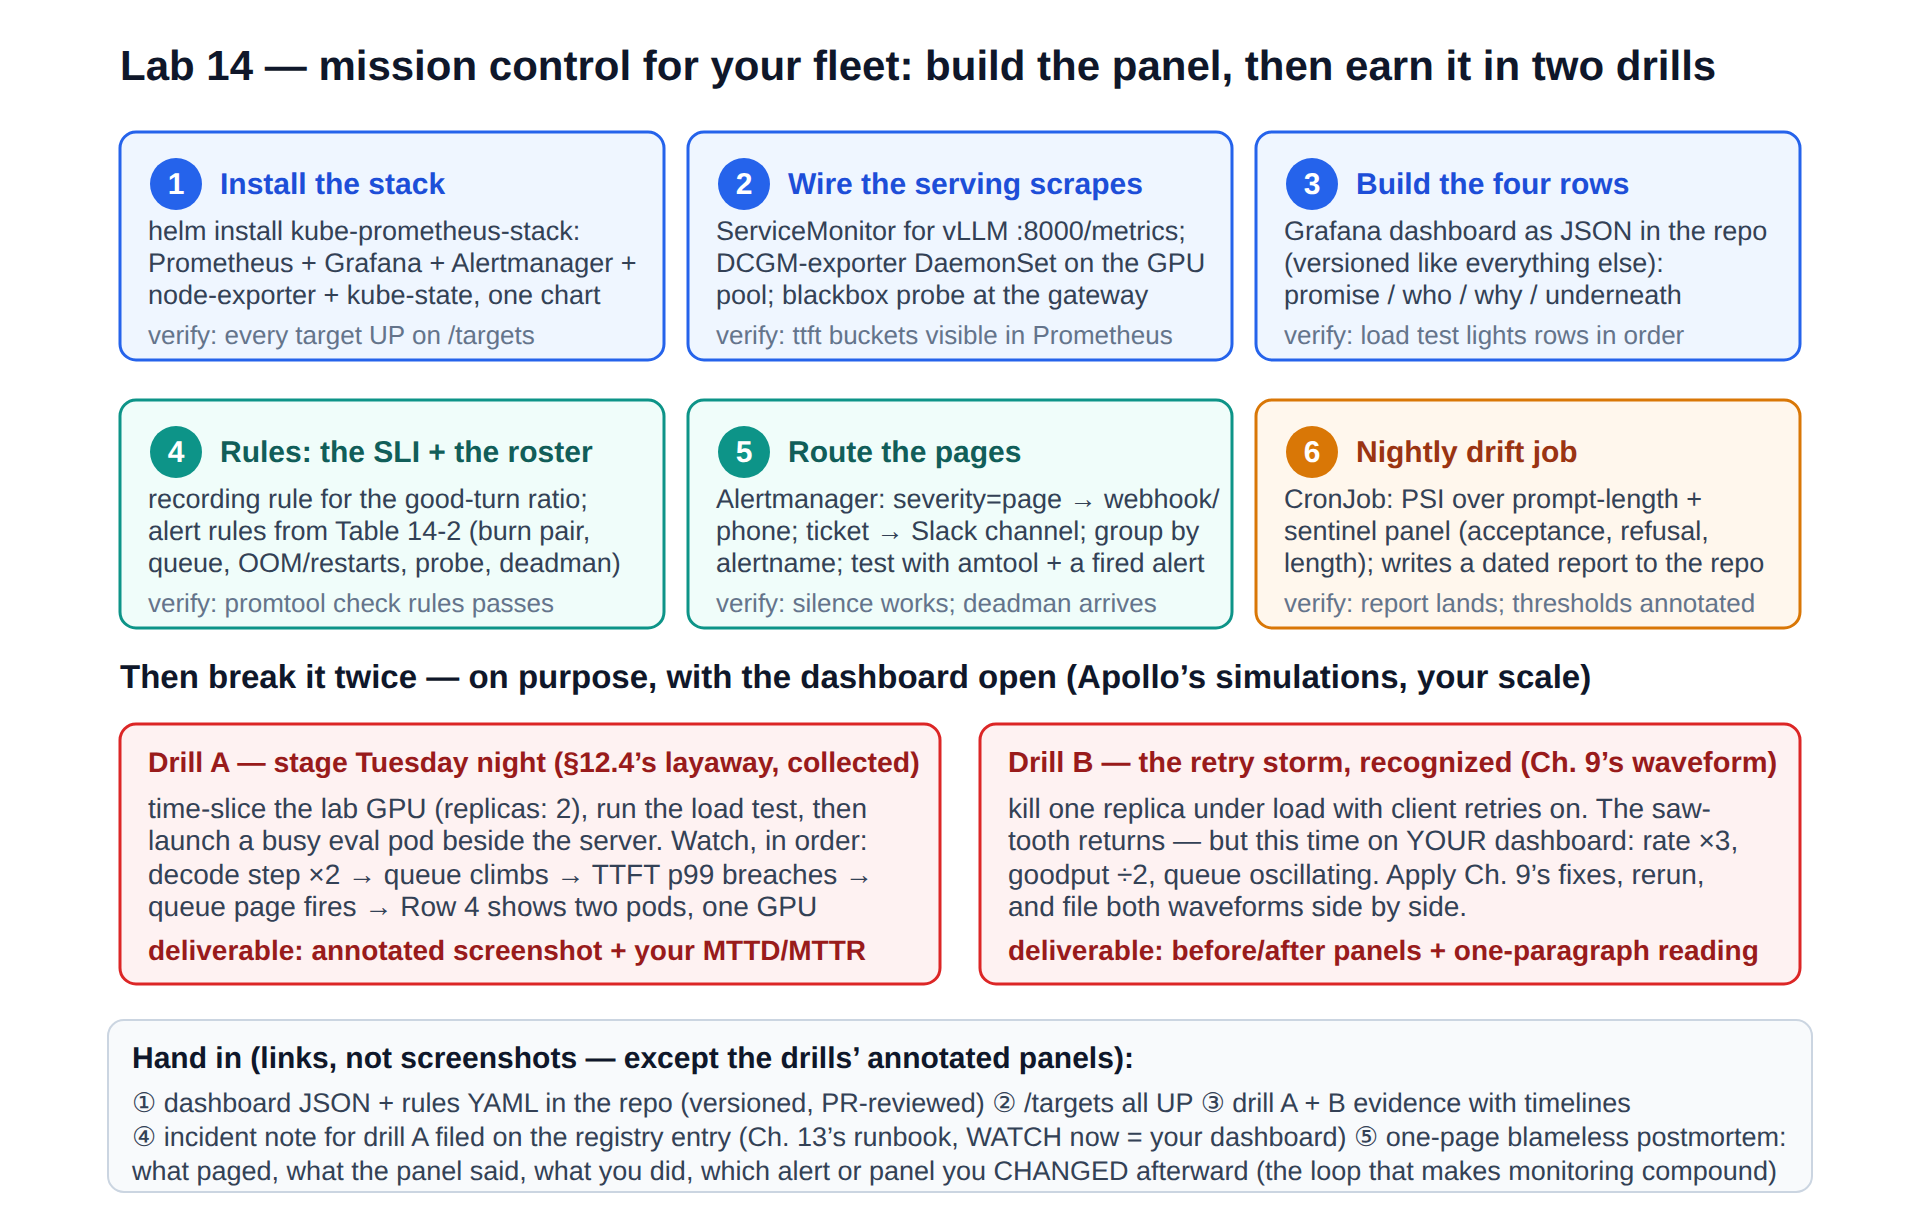
\includegraphics{figures/fig14-7_lab.png}}\\[3pt]
  \figcaption{그림 14-7  실습 14. 1–3단계에서는 stack을 세우고 네 행을 그리며, 4–5단계에서는 경보 목록을 작동시키고 page를 routing한다. 6단계에서는 drift job의 일정을 잡는다. 이어 drill A가 자기 hardware에서 화요일 밤을 재현해 §12.4의 외상을 갚고, drill B가 이번에는 계측 도구를 갖춘 채 제9장의 retry storm을 재생한다. 결과물은 link로 제출하며, 채점자가 받는 image는 주석을 붙인 drill screenshot 두 장뿐이다.}
\end{tbbfigure}

\textbf{1–3단계: Stack 세우기.} Helm으로 \code{kube-prometheus-stack}을 설치한다. Chart 하나에 Prometheus, Grafana, Alertmanager, node-exporter, kube-state-metrics가 들어 있다. 다른 일을 시작하기 전에 \code{/\allowbreak targets}에서 모든 target이 UP인지 확인한다. Scrape 점호가 실습의 첫 번째 정직한 결과물이며 \code{up == 0} 행이 첫 debugging 문제다. 흔한 원인은 ServiceMonitor가 찾는 port name이 Service에 없거나 selector가 namespace를 놓친 경우다. Engine \code{:8000/\allowbreak metrics}와 classifier를 위한 ServiceMonitor 두 개, GPU node의 DCGM DaemonSet, §14.4의 세 probe를 실행하는 blackbox exporter를 연결한다. 이어 \textbf{네 행 dashboard를 repository의 JSON으로} 만든다. 표 14-1의 panel과 약속을 측정하는 모든 panel의 SLO 선, 4행의 UUID별 pod 표, "높게 고정되는 것이 건강함", "busy ≠ yours"처럼 가르치는 caption을 넣는다. 11주 차 token-aware load test를 concurrency 세 단계로 실행하면서 행이 \textit{인과 순서대로} 켜지는지 확인한다. 먼저 3행의 queue, 다음 1행의 p99, knee를 넘으면 마지막으로 2행이 누군가 한 명이 아니라 모두의 문제임을 보여야 한다. 순서가 다르면 query가 틀렸다. 이제 dashboard가 스스로를 검사한다.

\textbf{4–6단계: 경보 작동시키기.} SLI recording rule과 표 14-2의 경보 목록을 code로 만든다. 사용자 한 명인 실습 환경에서는 플릿의 8이 아니라 터미널 기록 11-5에서 측정한 seat 수에 맞춰 queue threshold를 조정한다. CI에서 \code{promtool check rules}가 통과하는지 확인한다. Rule도 release artifact이므로 pipeline은 weights처럼 gate한다. Page는 전화와 가까운 receiver로 보낸다. 자기 device를 울리는 webhook이면 충분하다. Ticket은 channel로 보낸다. \code{amtool}로 synthetic alert를 발생시켜 grouping되고 silence가 유지되는지 확인해 연결을 입증한다. Dead man’s receiver는 \textit{cluster 바깥}에 세운다. Heartbeat service의 무료 tier나 lab VM의 cron이면 충분하다. 핵심은 운명을 공유하지 않는 데 있다. 10주 차 gate 실행으로 reference window를 고정하고 03:10에 drift CronJob을 예약한다. WATCH 판정을 포함한 첫 실제 report를 결과물과 함께 제출한다. 이제 채점하는 부분, 즉 \textbf{두 번 깨뜨리기}로 넘어간다.

\begin{terminalbox}
\begin{Verbatim}[breaklines=true,breakanywhere=true,fontsize=\small,formatcom=\color{tbbtermfg},codes=\tbbcodeactive]
# drill A -- stage tuesday night against your own server (lab GPU, qwen-1.5b)
$ kubectl patch cm nvidia-device-plugin -p '{"data":{"config":"replicas: 2"}}'
$ locust -f loadtest.py --headless -u 24 &          # steady load, seats full
$ kubectl create job eval-burn --image=... -- python soak.py --busy
# watch, in order (screenshot each transition):
#   row 3: decode step p50 0.021 -> 0.044   <- the neighbor's tax
#   row 3: num_requests_waiting 0 -> 11     <- the queue is local
#   row 1: TTFT p99 0.28 -> 2.9s; SLI ratio dives
#   21:0X  PAGE QueueSustained (your phone buzzes; note the clock)
#   row 4: pods-per-UUID: your-gpu: 2 (qwen-srv, eval-burn)
$ kubectl delete job eval-burn && date              # note the clock again
#   queue drains; page auto-resolves. MTTD = page - patch. MTTR = delete - patch.

# drill B -- week 9's retry storm, now with instruments (classifier pair)
$ locust -f storm.py --headless -u 60 &   # client retries ON (the bad config)
$ kubectl delete pod classifier-1         # kill one of two under load
#   rows: req rate x3 (retries multiplying), goodput /2, queue sawtooth --
#   the waveform from week 9, on YOUR panels. now apply ch. 9's fixes
#   (retry connect-only, one layer, jitter, shed early) and re-run:
#   same kill, flat goodput, no storm. file both panels side by side.
\end{Verbatim}
\end{terminalbox}
\figcaption{터미널 기록 14-6  두 가지 drill. Drill A는 자기 hardware에서 time-slice ConfigMap과 바쁜 이웃, 그림 14-4의 정확한 panel 순서를 재현해 §12.4의 외상을 갚는다. 자기 전화가 pager이고 벽시계가 채점자다. Drill B는 제9장의 storm을 재생해 waveform과 그것을 그리는 panel을 시각적 기억 속에 나란히 남긴다. 그 장에서 새벽 2시에 중요해질 것이라고 약속한 “Grafana screenshot 두 장”을 마침내 찍는다.}

\textbf{제출할 것}은 주석을 붙인 drill panel 두 장을 제외하면 screenshot이 아니라 link다. PR history가 있는 repository의 dashboard JSON과 rule YAML, \code{/\allowbreak targets} 점호, 그림 14-1의 12분과 8분에 견준 \textit{자기 MTTD와 MTTR}을 적은 drill A timeline, 한 문단 해설을 곁들인 drill B의 storm 전후 panel, drift job의 첫 report를 제출한다. 학기 전체를 묶는 결과물도 있다. 제13장 runbook을 사용해 \textbf{drill A의 incident note를 자기 registry 항목에 연결한다.} 이제 WATCH 줄에는 자기 dashboard 행의 이름이 들어간다. 한 페이지짜리 비난 없는 postmortem도 작성하며 action item에는 \textit{monitoring 자체의 변경}을 하나 이상 넣어야 한다. 새 alert, 수정한 threshold, 다음 새벽 2시의 두뇌에서 30초를 아껴 줄 caption이 예다. 마지막 요구 사항이 실습의 주장을 축소해 담고 있다. Monitoring stack은 정원과 같은 방식으로 완성된다. 일부러 절대 끝내지 않고 사고를 하나씩 겪으며 가꾼다.

\begin{calloutbox}{tbbamber}{tbbxFFFBEB}
{\normalsize\bfseries\color{tbbx92400E}상자 14-2  채점 기준 — 실습 14(감점되는 위험 신호 포함)}\par\vspace{3pt}
\begin{tbbitemize}
  \item \textbf{Stack + scrape(20\%).} 증거와 함께 모든 target이 UP이다. ServiceMonitor와 exporter는 손으로 적용하지 않고 repository에 둔다. 위험 신호: target이 0/N인데 그 metric을 query하는 dashboard, 즉 확신에 찬 빈 panel.
  \item \textbf{Dashboard 설계(25\%).} Runbook 순서로 네 질문에 답하는 네 행, 그려진 SLO 선, 모든 곳의 올바른 percentile 집계가 필요하다. Board 어디든 avg-of-p99s가 하나 있으면 이 항목은 절반이 상한이다. Caption은 사용법을 가르쳐야 한다.
  \item \textbf{경보 목록(20\%).} Recording rule을 읽는 burn 짝, 지속 조건을 둔 queue page, page가 아니라 ticket으로 보내는 원인, 처음부터 끝까지 검증한 deadman이 필요하다. 위험 신호: 정상적인 실습 traffic에서 매주 한 번보다 자주 page를 울릴 목록. 횟수를 직접 세고 밝힌다.
  \item \textbf{Drill(25\%).} 둘 다 직접 재현하고, 지켜보다가 알아차리는 대신 \textbf{자기} alert가 잡아야 한다. MTTD/MTTR을 측정해 정직하게 비교한다. Drill B는 실패가 일어나는 모습뿐 아니라 수정이 작동하는 모습도 보여야 한다. 위험 신호: 시계가 없는 screenshot.
  \item \textbf{순환 고리(10\%).} Registry 항목에 incident note를 연결하고 monitoring을 바꾸는 action item을 담은 postmortem을 PR로 배포한다. 실제 플릿을 잘 운영할 사람을 가장 잘 예측하는 기준이다.
\end{tbbitemize}
\end{calloutbox}

\begin{calloutbox}{tbbpurple}{tbbpurplefill}
{\normalsize\bfseries\color{tbbpurple}생각해 보기}\par\vspace{3pt}
\begin{tbbitemize}
  \item Time-sliced T4에서 drill A는 decode step을 약 2.1×로 만들지만 CPU의 classifier drill은 p50이 거의 움직이지 않는 동안 p99가 세 배가 된다(터미널 기록 12-4의 형태). 두 현상을 기본 원리로 설명하자. 각 workload는 어떤 resource를 포화시키며 time-slicing은 왜 median보다 tail에 먼저 세금을 부과하는가?
  \item Queue page threshold는 터미널 기록 11-5의 seat census에서 나왔다. 12주 차 autoscaler는 이제 매시간 레플리카 수를 바꾼다. Autoscaling에도 살아남는 threshold 식을 제안하자. 힌트: pod별 gauge와 플릿 합계 중 표 14-2는 무엇을 골랐으며 그 이유는 무엇인가? 반대로 선택할 때의 실패 형태도 말하자.
  \item Drill B의 나쁜 실행에서 처음 60초 동안 1행 SLI는 거의 움직이지 않았지만 3행은 비명을 질렀다. §14.4의 “증상은 page로, 원인은 ticket으로”와 조화시키자. Retry storm에서 queue sawtooth는 증상인가 원인인가? 답은 QueueSustained의 지속 window에 무엇을 요구하는가?
  \item Postmortem은 monitoring 변경을 요구한다. Drill A에서 나온 GPU UUID별 pod ticket, baseline 대비 decode-step 비율 panel, pool별 time-slice config expiry를 확인하는 CI 가운데 프로젝트 플릿에 가장 잘 일반화되는 변경 하나를 고르고 논증하자. 각 선택은 어떤 미래 사고 부류를 막지 못하는가?
\end{tbbitemize}
\end{calloutbox}

\namedsection{요약}{열여섯 가지로 정리한 이 장}

\qitem{1}{\textbf{두 번의 밤이 하나의 주장을 입증한다. 오후 2시에 그래프로 그린 것만 새벽 2시에 볼 수 있다.} 첫날 밤의 다섯 가지 확인은 모두 잘못된 질문에 정확히 답했다. 프로브는 살아 있는지 재고, 로그는 자백을 기록하며, 평균은 누구도 설명하지 못하고, 파드 하나는 일화일 뿐이며, GPU 사용률에는 누구의 작업이든 포함된다. 나쁜 사용자 시간은 85분이었다. 둘째 날 밤에는 같은 사람이 미리 준비한 질문으로 20분 만에 해결했다.}

\qitem{2}{\textbf{Apollo는 이 강의 계획서의 축소판이다.} 텔레메트리는 미리 설계하지 않으면 존재하지 않는다. 로켓이나 플릿에 ssh로 접속할 수는 없다. 원시 신호 자체가 아니라 \textbf{알아본 특징}이 사람을 구한다. SCE-to-AUX는 훈련에서 익힌 기억이었다. 착륙을 구한 요약표도 실패한 시뮬레이션 뒤에 작성되었다. 계측하고, 연습하고, 주석을 남겨라.}

\qitem{3}{\textbf{프로브는 반사 작용이고 모니터링은 기억이다.} 5장의 문장이 결실을 맺는다. 대시보드는 기억, 경보는 주의, 드리프트 모니터는 예견이다. 관측 가능성은 미리 정의하지 않은 질문에도 답할 수 있게 하는 속성이다. 화요일의 충돌을 위한 전용 패널은 없었지만 범용적인 네 행이 답을 찾아냈다.}

\qitem{4}{\textbf{세 기둥은 비용이 생기는 방식이 다르다.} 지표는 시계열마다 비용을 내며 저렴하고 항상 켜져 있다. 경보는 여기에 둔다. 로그는 이벤트마다 비용을 내는 파드의 전기이며, 6장의 대가를 치른 덕분에 파드가 죽기 \textit{전에 파드 밖으로} 보낸다. 트레이스는 요청마다 비용을 내고 표본을 추출하며, 홉이 세 개인 이 강좌에서는 최소한으로 쓴다. 5장에서 예고한 수행원 가운데 익스포터와 로그 전송기는 설치하지만, 관심사마다 소유자를 하나만 두기 위해 메시는 보류한다.}

\qitem{5}{\textbf{지표는 이름 + 레이블 + 값 + 시각이며, 비용은 시계열 단위로 낸다.} 레이블은 파드, UUID, 경로처럼 한정된 목록에서 “어느 것인가?”에 답한다. 사용자나 요청처럼 값이 무한히 늘어나는 정보는 로그에 둔다. 카디널리티(cardinality)는 모니터링의 메모리 장벽이다. 부주의한 레이블 하나가 시계열 14,000개를 천 배로 늘린다.}

\qitem{6}{\textbf{형태는 셋이지만 명령은 하나다.} 카운터는 오르기만 하므로 rate()로 변화율을 구하며 재시작에도 안전하다. 게이지는 지금 값을 읽으며 포화를 표현한다. 히스토그램은 \textbf{백분위수의 평균을 낼 수 없기 때문에} 존재한다. 버킷 카운터는 레플리카에 걸쳐 더할 수 있고, 합친 버킷의 백분위수만 올바른 플릿 p99다. p99의 평균은 2.76 s라고 했지만 실제 값은 9.08 s였다.}

\qitem{7}{\textbf{부재도 사실이어야 하므로 풀 방식을 쓴다.} 스크레이프마다 up\{pod\}를 기록하고, 죽은 대상은 침묵 대신 묘비를 남긴다. 계보는 Borgmon에서 Prometheus로 이어졌다. Prometheus는 2012년 SoundCloud에서 시작해 Kubernetes에 이어 CNCF의 두 번째 프로젝트가 되었다. Grafana는 2014년에 Kibana를 포크해 출발했다. 기록 규칙은 SLI를 미리 계산하며 13장의 파이프라인으로 배포한다. 규칙도 릴리스 산출물이다.}

\qitem{8}{\textbf{익스포터 모음은 강좌 전체를 다시 관통한다.} node-exporter는 2장의 머신을, cAdvisor는 바깥에서 cgroup 파일을 읽어 3장의 정직한 마운트를 구현한다. 이제 memory.events의 oom\_kill과 memory.high 경보도 그래프로 볼 수 있다. kube-state는 재시작, OOMKilled, 엔드포인트, 롤아웃 상태 등 5장의 경보 목록을 제공한다. DCGM은 nvidia-smi를 산업 규모로 확장해 UUID별 값을 파드와 조인한다. 엔진의 /metrics에는 11장의 선들이 있고, 블랙박스는 6장의 출입구를 바깥에서 조사한다.}

\qitem{9}{\textbf{GPU “사용률”은 점유 듀티 사이클일 뿐이다. 바쁨 ≠ 내 것 ≠ 효율적임이다.} 메모리 병목 디코드는 ALU의 10분의 1만 쓰면서도 90\%+로 표시될 수 있고, 테넌트 둘이 함께 쓰면 둘 다 \textasciitilde{}100\%로 보인다. 그 값만으로는 누구의 작업인지 알 수 없다. 대기열, 선점, DRAM 활동 같은 포화 신호가 먼저 나타나고, 사용률은 뒤처지며 오해를 부른다. 자원에는 USE, 서비스에는 RED를 적용하고, 대기열을 핵심 포화 게이지로 삼는다.}

\qitem{10}{\textbf{네 행 대시보드는 약속 → 누구 → 원인 → 기반의 순서다.} 1행은 오류 예산, 소진율, 올바른 p99, 스트림별 속도로 SLO 문장을 패널에 옮기며 호출을 보내는 유일한 행이다. 2행은 레플리카별 RED로 모두가 느린지 일부만 느린지 가른다. 3행은 대기열, 높게 고정되어 정상인 KV, 디코드 속도, 선점으로 엔진 내부의 원인을 보여 주며 9장의 대기열/계산 분리를 지킨다. 4행은 UUID별 DCGM, GPU당 파드, 오토스케일러 태세로 기반을 보여 준다.}

\qitem{11}{\textbf{증상에는 호출을, 원인에는 티켓을 보낸다.} 증상은 적고 실제이며 완전하다. 처음 보는 실패도 SLI에 드러난다는 사실을 충돌 사고가 입증했다. 원인은 셀 수 없이 많고 값싸며 해가 없는 경우도 흔하다. 병원에서는 경보의 85–99\%에 조치가 필요 없었고, 경보 피로가 사람을 죽인다는 대가를 배웠다. 모든 호출은 조치할 수 있고, 긴급하며, 실제여야 한다.}

\qitem{12}{\textbf{SLO 문장은 소진율로 컴파일된다.} p99 ≤ 500 ms ≡ 99\% of turns good → SLI ratio → budget = 1\% × \textasciitilde{}9.5M turns ≈ 95k bad turns/30 d라는 식으로 이어진다. Burn = bad-fraction ÷ 0.01이다. 다중 구간 정책은 14.4×/1 h∧5 m이면 호출, 6×/6 h이면 호출, 3×/1×이면 티켓을 만든다. 긴 구간은 의심하고 짧은 구간은 용서한다. 대기열 같은 선행 증상에는 빠른 경로를 허용한다.}

\qitem{13}{\textbf{거부할 수 있는 모든 계층의 바깥에 서라.} 출입구, 응답, 스트림을 검사하는 세 합성 프로브(synthetic probe)는 각각 자신이 지목할 계층 바깥에 있어야 하고, 실패의 존재가 아니라 지속성에 호출을 보낸다. 사례 14-A의 초록색 /health는 첫 번째 프로브 하나뿐이었다. Watchdog는 항상 발화하므로 그 침묵을 경보로 삼는다. 클러스터와 운명을 공유하지 않는 수신기가 침묵을 감지해 호출을 보낸다. 데드맨 스위치(dead man's switch)가 감시자를 감시한다.}

\qitem{14}{\textbf{사람이 참여하는 순환은 모니터링의 가치를 복리로 키운다.} 호출에는 WATCH 단계에서 대시보드 행을 지목하는 런북이 붙는다. 사고는 사람 이름이 아니라 메커니즘을 다루는 비난 없는 사후 분석으로 끝나며, 조치 항목은 반드시 \textbf{모니터링을 바꾼다}. 화재가 날 때마다 연기 감지기가 하나씩 생긴다. 메모는 레지스트리 항목에 등록되어 마침내 10장의 검토자가 읽는다. MTTD와 MTTR은 이 순환을 채점하고 DORA의 네 번째 핵심 지표를 완성한다. 스택 비용은 \textasciitilde{}\$23/mo이며 원장은 정확히 \$900에 마감된다.}

\qitem{15}{\textbf{드리프트는 호출을 보내지 않는 실패다. 카나리는 절벽을 잡고 드리프트 모니터는 경사를 잡는다.} 대응 방식에 따라 데이터 드리프트(data drift), 개념 드리프트(concept drift), 사전 확률 변화, 평가 세트 노후화로 나눈다. 데이터 드리프트에서는 입력이 움직여 서빙 계산과 평가 범위가 먼저 깨진다. 개념 드리프트에서는 정답이 움직여 최신 현실을 반영한 평가만 이를 발견한다. 사전 확률 변화에서는 작업 구성이 달라져 가드레일 기준선을 다시 잡아야 한다. 평가 세트도 낡으므로 분기마다 다시 표본을 뽑는다. 수락률, 거부율, 길이, 프리필 p50 같은 감시 지표(sentinel metric)는 추가 비용 없이 얻는다. PSI는 손으로 계산할 수 있으며 0.144는 관찰 구간이다. 경사에는 호출이 아니라 \textbf{검토}를 배정한다.}

\qitem{16}{\textbf{대응 사다리는 반응 비용을 정한다.} 관찰 → 새로운 표본으로 재평가 → 서빙 다시 조정 → 13장의 레지스트리→게이트→카나리를 거치는 새 후보 순으로 올라간다. 판정기는 이미 약정한 비용 범위에서 유휴 골짜기를 활용하므로 Insull의 얼음 창고처럼 한계비용이 0달러다. 운영 데이터가 다시 개발로 흘러가며 1장의 순환이 닫힌다. 어떤 PSI도 계산하지 못하는 월요일의 질문도 남는다. 지금도 이 약속이 올바른 약속인가?}

\namedsection{연습문제}{}

\subsection*{A. 객관식}

\qitem{1}{첫날 밤의 다섯 가지 확인(프로브, 로그, 평균, 파드 하나의 p99, nvidia-smi)이 실제 장애 중에도 모두 “통과”한 이유는?}

\begin{tbboptions}
  \item ① 도구 설정이 잘못되었다.        ② 각 도구는 생존, 자백, 중심 경향, 일화, 점유처럼 SLO와 다른 질문에 답하며 약속 자체를 계산한 도구는 하나도 없었다.
  \item ③ 사고가 너무 짧아 관측할 수 없었다.        ④ 플릿에 레플리카가 충분하지 않았다.
\end{tbboptions}

\qitem{2}{레플리카 네 개의 p99를 평균 내면 2.76 s지만 실제 플릿 p99는 9.08 s다. 근본적인 오류는?}

\begin{tbboptions}
  \item ① 구간이 너무 짧었다.        ② 백분위수는 선형이 아니므로 합친 분포의 분위수만 의미가 있으며, 레플리카에 걸쳐 더할 수 있는 것은 버킷 카운터뿐이다.
  \item ③ rate()를 빠뜨렸다.        ④ 버킷 경계가 SLO와 맞지 않았다.
\end{tbboptions}

\qitem{3}{DCGM\_FI\_DEV\_GPU\_UTIL 값이 93\%다. 이 값으로 실제로 알 수 있는 사실은?}

\begin{tbboptions}
  \item ① GPU가 포화 상태의 93\%에 도달했다.        ② 내 파드가 FLOP의 93\%를 사용한다.
  \item ③ 최근 시간의 93\% 동안 누구의 것이든 커널 하나 이상이 올라와 있었다. 점유 듀티 사이클일 뿐 여유 용량, 효율, 소유권은 알려 주지 않는다.        ④ 이웃이 쓸 수 있는 용량이 7\% 남았다.
\end{tbboptions}

\qitem{4}{Garman이 말한 “너무 자주 반복되지 않으면 진행한다”는 판단은 이 장의 체계에서 무엇에 해당하는가?}

\begin{tbboptions}
  \item ① 침묵        ② 심각도 사다리        ③ 데드맨 스위치        ④ 발생률과 지속성에 따른 경보. for:, 지속 구간, 짝을 이룬 소진 구간을 이용해 존재 자체가 아니라 반복에 호출을 보낸다.
\end{tbboptions}

\qitem{5}{99\% / 30-day SLO에서 소진율이 24×라는 뜻은?}

\begin{tbboptions}
  \item ① 요청의 24\%가 SLO 임곗값을 위반하며, 이 속도면 월간 예산이 \textasciitilde{}30 h (30 d ÷ 24) 만에 소진된다.        ② SLO가 24× 지나치게 엄격하다.
  \item ③ p99가 임곗값의 24×다.        ④ 호출기가 24번 울린다.
\end{tbboptions}

\qitem{6}{소진율 호출이 완전성을 보장하는데도 QueueSustained 호출을 따로 두는 이유는?}

\begin{tbboptions}
  \item ① 소진율 규칙은 신뢰할 수 없다.        ② 대기열은 원인이며 원인에도 호출을 보내야 한다.
  \item ③ 소진율이 24×여도 1시간 구간이 14.4×를 넘는 데 약 35분이 걸린다. 대기열은 선행 증상이므로 증상에는 빠른 경로를 허용한다.        ④ Alertmanager는 두 호출을 라우팅할 수 없다.
\end{tbboptions}

\qitem{7}{Watchdog 경보는 vector(1)을 평가해 계속 발화한다. 그 이유는?}

\begin{tbboptions}
  \item ① 호출기를 예열한다.        ② 외부 수신기에서 이 경보가 사라지는 것 자체가 경보다. 심장박동이 멈추면 모니터링 스택이 죽었다는 뜻이며, 이것이 데드맨 스위치다.
  \item ③ Prometheus에는 활성 경보가 하나 필요하다.        ④ 경보 지연 시간을 측정한다.
\end{tbboptions}

\qitem{8}{야간 작업이 프롬프트 길이 PSI = 0.144를 보고했고 여러 감시 지표도 같은 방향으로 움직인다. 올바른 대응은?}

\begin{tbboptions}
  \item ① 당직자를 호출한다.        ② 즉시 다시 학습한다.        ③ 관찰 구간(0.1\textasciitilde{}0.25)이므로 주간 검토를 하고 새로운 표본 평가인 사다리 2단계로 올린다. 경사에는 호출이 아니라 검토를 배정한다.        ④ SLO 임곗값을 높인다.
\end{tbboptions}

\subsection*{B. 단답형}

\qitem{1}{플릿의 TTFT p99를 구하는 PromQL을 작성하고 세 계층(rate, sum by le, histogram\_quantile)이 각각 기여하는 바를 설명하라. 가장 안쪽 계층이 재시작에도 안전한 이유도 포함하라.}

\qitem{2}{KV 캐시 사용률은 96\%에 고정되어도 경보가 울리지 않지만 num\_requests\_waiting이 6분 동안 9를 유지하면 사람을 깨운다. 11장의 아키텍처를 근거로 두 설계를 정당화하라. 각 게이지가 무엇을 측정하며, 어느 것이 수요가 좌석을 초과했음을 뜻하는가?}

\qitem{3}{세 합성 프로브의 경로, 실행 빈도, 경보 조건을 명시하라. 각 프로브가 거울이 아니라 목격자가 되려면 어느 계층 바깥에 있어야 하는지도 설명하고, 가장 먼저 발견하는 6장의 실패 유형(503 / 504 / 스트림 끊김)에 대응시켜라.}

\qitem{4}{7장의 99.9\%는 43분을 허용했고 이 장의 99\%는 95,000턴을 허용한다. 요청 기반 단위가 시간 기반 단위와 달리 하루 주기 물결의 비용을 올바르게 매기는 이유를 설명하라. 새벽 3시와 21시 30분의 나쁜 1분은 두 회계 방식에서 각각 얼마의 비용이 되는가?}

\qitem{5}{각 항목을 호출 또는 티켓으로 분류하고 한 절씩 근거를 제시하라. (a) 준비된 엔드포인트 = 0, (b) 프로덕션 UUID당 파드 = 2, (c) probe\_success가 3× 연속 실패, (d) 레플리카 하나에서 OOMKilled 한 번 관측, (e) 6 h 동안 소진율 6×, (f) 10 min 동안 선점률 0.8/s.}

\qitem{6}{수락률 감시 지표를 설명하라. 초안 수락률 하락이 입력 분포의 온도계인 이유, 어떤 비용이 다른 어떤 비용보다 먼저 나타나는지, 신호를 가장할 수 있는 교란 요인, 이를 구분하는 레지스트리 질의를 모두 다루어라.}

\subsection*{C. 논술형}

\qitem{1}{화요일 사고의 비난 없는 사후 분석을 작성하라. 두 경보, 대시보드 조사, 퇴출을 분 단위 연표로 정리하고, 첫날 밤의 반사실(20분 대 85분)을 이용해 나쁜 사용자 시간으로 영향을 계산하라. 사람 이름이 아니라 메커니즘, 즉 오래된 시분할 ConfigMap과 빠진 UUID당 파드 정책으로 근본 원인을 서술하라. 담당자가 있는 조치 항목 세 가지를 제시하되 적어도 하나는 모니터링 자체를 바꾸어야 한다. 대부분의 사후 분석이 빠뜨리는 문단, 즉 이 사고가 새로 만들 근거가 \textit{되지 못하는} 것은 무엇이며 왜 그런지도 덧붙여라.}

\qitem{2}{정상 상태에서 월 2회라는 명시적 경보 피로 예산 아래 프로젝트 플릿의 전체 호출 정책을 설계하라. 직접 측정한 트래픽, 좌석 수, 도착률을 근거로 심각도와 구간을 정한 경보 목록, 데드맨의 외부 수신기, 그룹화와 억제 규칙을 포함하라. 감사자가 가장 먼저 읽을 부분도 작성하라. 어떤 실패 유형을 의도적으로 티켓으로 낮췄으며, 각 결정으로 어느 정도의 사용자 고통을 받아들이는가?}

\qitem{3}{“모니터링은 카나리의 분석 구간을 영구화한 것이다.” 13장의 금요일 버그에서 답변 길이를 따라 카나리 가드레일, 기록 규칙, 드리프트 감시 지표까지 추적하라. 각 시간 척도에 대해 구간, 임계값 방식(고정값, 기준선 대비, 기준 분포 대비), 독자, 대응을 제시하라. 같은 숫자가 세 계측 도구에 모두 쓰이는 이유와, 어떤 지표만 존재할 가치가 있는지에 관한 함의도 논증하라.}

\qitem{4}{관측 비용에 관한 논술이다. 23달러 항목, TSDB 대략 계산, 판정기의 유휴 골짜기 활용, 가장 희소한 자원인 당직자의 주의를 포함해 모니터링 스택의 비용을 정직하게 계산하라. 이 규모의 플릿에서 관측 가능성의 한계가치와 한계비용이 만나는 지점을 찾는다. 그런 다음 오류 예산 패널, 사전 합의한 완화 조항, 런북을 이용해 7장의 새벽 2시 논술 문제를 해결하고 다음 주장에 찬성하거나 반박하라. “지루한 운영이 이 강좌 전체의 올바른 최종 상태이며, 23달러는 청구서에서 가장 저렴한 항목이었다.”}

\namedsection{정답과 해설}{}

\subsection*{A. 객관식}

\qitem{1}{\textbf{②} 정직한 계측 도구는 다섯 개였지만 이를 조합한 곳은 없었다. SLO가 정의한 “정상”, 즉 SLI를 어디에서도 계산하거나 분해하지 않았다. 1행이 약속을 확인하는 다섯 도구를 대신하고 2\textasciitilde{}4행이 원인 탐색을 대신한다. (§14.1)}

\qitem{2}{\textbf{②} 꼬리 값의 평균은 허구다. 9.8 s인 레플리카 하나와 0.4 s인 레플리카 세 개를 평균 내면 아무도 실제로 겪지 않은 지연 시간이 나온다. 합친 버킷 자체가 플릿 분포다. 이는 7장의 네 번째 문법 규칙을 도구로 강제한 것이다. (§14.2)}

\qitem{3}{\textbf{③} 누구의 것이든 커널 하나가 올라와 있던 시간의 듀티 사이클이다. 메모리 병목 디코드 루프는 ALU를 굶기면서도 이 값을 높게 고정할 수 있고, 이웃의 커널도 계산에 포함된다. 여유 용량은 포화와 PROF\_* 지표에서, 소유권은 UUID당 파드 조인에서 찾는다. (§14.2)}

\qitem{4}{\textbf{④} 1202 경보는 간헐적이었고 유도 장치는 계속 작동했다. 하강 전에 문서로 정한 발생률 조건과 증상 확인을 함께 적용한 것이다. for:, 지속 평균, 짝을 이룬 구간은 이 판단을 자동화한 형태다. (§14.4)}

\qitem{5}{\textbf{①} Burn = bad-fraction ÷ (1 − SLO) = 0.24 ÷ 0.01이고, time-to-empty = 30 d ÷ burn이다. 핵심 관점은 소진율이 예산의 \textbf{지출 속도}라는 것이다. 그래서 여러 속도의 정책을 일관되게 구성할 수 있다. (§14.4)}

\qitem{6}{\textbf{③} 긴 구간이 의심하는 동안 지연이 생긴다. 소진율 24×에서도 35 min이 든다. 용량 문제로 생긴 고통은 7장의 무릎점과 11장의 허용 선처럼 대기열에서 먼저 드러나므로, 증상 빠른 경로는 \textasciitilde{}7분 만에 호출한다. 둘 다 증상이며, 원칙주의적 반론은 생각해 보기 상자에서 다룬다. (§14.4)}

\qitem{7}{\textbf{②} 침묵을 경보로 삼으면 실패 방식이 뒤집힌다. 죽은 Prometheus는 자신의 죽음을 호출할 수 없으므로, Prometheus가 죽일 수 \textbf{없는} 대상인 외부 수신기가 호출해야 한다. 리전, 결제, 웹훅(webhook) 체인을 별도로 감사해 클러스터와 운명을 공유하지 않게 한다. (§14.4)}

\qitem{8}{\textbf{③} 드리프트는 경사다. 경사에 호출을 보내면 경보 피로가 다시 생긴다. 관찰 판정은 새로운 표본을 유휴 골짜기에서 평가하는 2단계를 예약하고 보고서를 레지스트리 항목에 등록하며, 정기 검토 주기에 사람이 참여하게 한다. (§14.5)}

\subsection*{B. 단답형}

\qitem{1}{histogram\_quantile(0.99, sum by (le) (rate(vllm:time\_to\_first\_token\_seconds\_bucket[5m]))). rate()는 누적 버킷 카운터를 초당 흐름으로 바꾸고 카운터 초기화를 이어 계산한다. 파드가 다시 태어나면 초기화로 나타나지만 이를 감지하고 보정한다. 그렇지 않으면 5장의 조정 과정이 모든 그래프를 오염시킨다. sum by (le)는 버킷 경계를 보존하면서 레플리카를 합치는 유일하게 올바른 교차 레플리카 집계다. histogram\_quantile은 해당 버킷 안에서 분위수를 보간하므로 오차는 버킷 너비 정도다. (§14.2)}

\qitem{2}{KV 풀은 캐시 형태의 \textbf{할당}이다. PagedAttention의 설계 목표는 풀을 가득 채우는 것이다. 좌석이 가중치 스트림 비용을 분산하므로 높게 고정된 상태는 머신이 제값을 하는 상태다. 3장의 페이지 캐시 교훈을 GPU에 적용한 것이다. 대기열은 \textbf{허용}을 측정한다. 대기가 지속되면 도착률이 좌석 처리량을 넘어 용량을 초과했다는 뜻이고, 사용자는 이미 TTFT로 비용을 치르고 있다. 한 게이지가 가득 차면 작동 중이고, 다른 게이지가 0보다 큰 상태로 지속되면 실패 중이다. (§14.2, 11장)}

\qitem{3}{출입구: 로드 밸런서 밖에서 30 s마다 HTTPS GET /v1/models를 보내고 3× 연속 실패하면 호출한다. 플릿이 볼 수 없는 경계 밖에 있으므로 TLS, 대상 상태, 라우팅과 같은 503 유형을 잡는다. 응답: 게이트웨이 밖에서 60 s마다 토큰 1개 완성을 요청하고 시간 제한은 10 s로 둔다. 출입구를 지난 뒤 허용이나 엔진에서 생기는 504/멈춤을 잡는다. 스트림: 5 min마다 짧은 스트리밍 완성을 요청해 첫 토큰이 ≤ 2 s이고 마지막 청크가 온전한지 확인한다. 유휴 시간 제한 계층 바깥에서 표 6-3 셋째 행의 스트림 끊김을 잡는다. 공통 규칙은 검사하는 계층 안의 프로브는 목격자가 아니라 거울이라는 것이다. (§14.4, 6장)}

\qitem{4}{시간 기반 예산은 모든 분에 같은 가격을 매기지만 계단형 수요는 그렇지 않다. 12장의 물결에서 새벽 3시의 1분에는 21시 30분의 약 3분의 1에 해당하는 턴만 들어온다. 요청 기반 예산은 사용자 단위로 지출한다. 화요일 피크 시간 20분의 비용은 \textasciitilde{}24\% × 23/s × 1,200 s ≈ 6.6k bad turns (7\% of the month)다. 시간 기반 회계는 고통받는 사람이 3분의 1뿐인 새벽 3시에도 같은 비용을 기록한다. 호출의 긴급도는 고통받는 사람 수를 따라야 하므로 턴을 사용한다. (§14.4)}

\qitem{5}{(a) \textbf{호출} — 라우팅할 곳이 없어 모든 사용자가 지금 503을 본다. (b) \textbf{티켓} — 원인이며 개발 환경에서는 해가 없지만 증상이 발생하면 결정적인 맥락이 된다. (c) \textbf{호출} — 이를 알 수 있는 유일한 외부 관점에서 출입구가 실제 사용자를 거부한다. (d) \textbf{티켓} — OOM 한 번은 5장의 완충된 사고이며, 플릿 전체에서 나타나 시스템 한도 오류가 되었을 때만 호출한다. (e) \textbf{호출} — 6 h 동안 6×인 느린 누출은 빠른 규칙에 걸리지 않으므로 이를 위해 짝 구간을 둔다. (f) \textbf{티켓} — 흔히 드리프트가 다가오며 생기는 풀 압력이므로 근무 시간에 조사한다(§14.5). (§14.4)}

\qitem{6}{수락률은 작은 초안 모델이 실제 트래픽을 얼마나 잘 예측하는지 추정한다. 요청마다 무료로 갱신되는 분포 일치 측정기다. 입력이 움직이면 초안이 먼저 틀리고, 품질 변화가 눈에 보이기 전에 TPOT가 초안 없는 하한으로 나빠져 \textbf{비용} 회귀가 먼저 나타난다. 올바른 순서로 도착하는 조기 경보다. 초안 모델이나 엔진 업데이트도 수락률을 움직일 수 있다는 교란 요인이 있다. 추세가 시작된 날 릴리스 세 요소의 다이제스트가 바뀌었는지 레지스트리 계보로 구분한다. 교란 여부와 관계없이 감시 패널에 둘 가치가 있지만, 판정이 아니라 합창의 한 목소리로 사용한다. (§14.5, 11장)}

\subsection*{C. 논술형(채점 기준)}

\qitem{1}{확인할 내용: 티켓이 11분 먼저 발생했음을 짚은 두 경보의 연표, 반사실인 85분을 단순 주장하지 않고 논증해 턴과 사용자 시간으로 계산한 영향, 소유자와 만료가 없는 오래된 ConfigMap 및 빠진 배치 정책이라는 메커니즘, 엔지니어 개인을 명시적으로 비난에서 제외한 서술, 서로 다른 종류의 조치 세 가지다. 경보를 정책으로 승격하고 CI에 만료 검사를 추가하고 캡션을 수정하는 식으로, 각각 담당자와 날짜가 있어야 한다. “만들지 않을 것” 문단이 답안의 수준을 가른다. 예를 들어 모든 곳에 파드별 반친화성을 강제하면 §12.4에서 정당하게 공유하는 개발 풀이 깨지고, 전용 이상 감지기는 §14.5의 함정이다. 느낌이 아니라 비용으로 판단해야 한다. (§§14.1\textasciitilde{}14.4)}

\qitem{2}{예산이 실제 선택을 강제한다. 측정한 트래픽을 바탕으로 규칙마다 예상 월간 발화 횟수를 \textbf{세고}, 이를 합해 2와 비교한 경보 목록을 높이 평가한다. 호출의 핵심에는 소진율 쌍, 선행 증상 하나, 출입구 프로브가 있어야 한다. 데드맨은 외부에 두고, 사고 하나가 호출 하나가 되도록 그룹화하며, 억제 규칙은 Watchdog에 절대 적용하지 않는다. 실패 유형을 낮춘 부분이 논술의 핵심이다. 레플리카 하나의 OOM을 티켓으로 낮추면 재시작 한 바퀴만큼의 지연을 받아들이게 되고(§3.6/§5.6 계산), 선점 급증을 티켓으로 낮추면 검토 전까지 TTFT가 천천히 악화되는 것을 받아들인다. 받아들인 고통을 \textbf{수치화}해야 만점을 받을 수 있다. (§14.4)}

\qitem{3}{흐름은 다음과 같다. 금요일에는 답변 길이가 몇 분 만에 211→54로 바뀌었고, 30\% 고정 가드레일을 카나리 컨트롤러가 읽어 자동 후퇴했다(13장). 기록 규칙은 영구적으로 5분 구간을 계산하고 이동 기준선 대비 임계값을 2행과 당직자가 읽어 조사한다. 드리프트 감시 지표는 게이트 구간의 기준과 21일 추세를 PSI 방식 구간으로 비교하며 월요일 검토자가 보고 대응 사다리를 밟는다. 좋은 답안은 불변 요소를 짚는다. 숫자 하나를 세 \textbf{구간}과 세 대응 속도에서 사용한다. 여러 시간 척도에서 쓸 수 있는 지표만 내보낼 가치가 있다는 결론으로 이어진다. 가드레일은 영속성을 얻지만 허영 지표는 두 번째 계측 도구를 얻지 못한다. (§§14.3\textasciitilde{}14.5, 13장)}

\qitem{4}{정직한 원장은 스택 23달러 + 유휴 골짜기를 쓰는 판정기 약 0달러 + 보존 기간으로 제한된 TSDB 증가분을 기록하고, 제약 자원인 당직자의 주의와 비교한다. 클라우드 청구서에 없어도 경보 피로는 \textbf{비용}이다. 추가 패널과 경보의 한계 신호로 조치할 수 없게 되는 순간 더 이상 비용을 정당화하지 못한다. 상자 14-1의 죄악은 그 지점을 넘었다는 증상이다. 새벽 2시 재현에는 1행의 예산 그래프와 7주차 문서에서 미리 합의한 완화 조항을 인용하고 “계산과 서명”에 도달해야 한다. 주장을 옹호하는 좋은 답안은 지루함 = 자동화 + 버전 관리 + 점진성 + 가역성(13장) + \textbf{관측됨}(14장)을 추적하고, 23달러로 첫 사고부터 둘째 날 밤의 차이인 사용자 시간 65분을 샀음을 지적한다. 반박하는 좋은 답안은 지루함이 작업이 아니라 운영의 속성이며, 흥미로운 문제는 드리프트, 평가, 제품처럼 스택 위로 이동했음을 지적한다. 어느 입장이든 계산이 일관되면 최고 등급을 받는다. (§14.4, 장 전체)}

\namedsection{더 읽을거리}{}

\textbf{[이번 주]} 표시는 실습에 직접 도움이 되는 자료이고, \textbf{[N주차]} 표시는 뒤에서 활용할 자료다.

\begin{tbbitemize}
  \item \textbf{[이번 주] Google SRE Book, 6장 “Monitoring Distributed Systems” + SRE Workbook, 5장 “Alerting on SLOs”} — 네 가지 황금 신호, 증상/원인 원칙, 표 14-2가 그대로 채택한 다중 구간·다중 소진율 정책을 다룬다. 그림 14-5를 옆에 두고 Workbook의 해당 장을 읽어 보라. 숫자가 의도적으로 일치한다.
  \item \textbf{[이번 주] Rob Ewaschuk, “My Philosophy on Alerting”} — “호출은 조치할 수 있고, 긴급하며, 실제여야 한다”라는 원칙의 씨앗이 된 짧은 문서다. 증상에는 호출을, 원인에는 티켓을 보낸다는 현대적 원칙도 여기서 시작되었다. 20분을 투자하면 경력 내내 보상을 얻는다.
  \item \textbf{[이번 주] Prometheus 문서의 “Histograms and summaries”, “Querying basics”와 Robust Perception 블로그} — 버킷 설계, 요약을 집계할 수 없는 이유, §14.2에서 다룬 날카로운 모서리, rate()의 미묘한 동작을 설명한다. Brian Brazil의 블로그에는 이 분야의 구전 지식이 글로 축적되어 있다.
  \item \textbf{[이번 주] kube-prometheus-stack 차트 문서 + Grafana 대시보드 모범 사례 + NVIDIA DCGM-exporter README} — 실습에서 설치할 세 구성 요소의 문서다. DCGM README의 지표 표에는 사용률의 세부 의미와 PROF\_* 계열이 있으며, 파드 매핑 절은 4행의 결정적 증거를 가능하게 한다.
  \item \textbf{D. Sculley 외, “Hidden Technical Debt in Machine Learning Systems” (NeurIPS 2015)} — §14.5에서 모니터링하는 얽힘, 피드백 루프, 고정된 모델 아래에서 변하는 세상에 이름을 붙인 논문이다. “monitoring and testing” 절은 마지막에 읽어 보라. 이 장의 내용을 10년 먼저 네 문단으로 압축해 두었다.
  \item \textbf{Chip Huyen, Designing Machine Learning Systems, 8장(“Data Distribution Shifts and Monitoring”)} — 이 강좌가 PSI 설명에 압축한 구간, 기준, 계절성과 같은 추정의 미묘함을 포함해 드리프트 분류를 책 한 장 깊이로 다룬다.
  \item \textbf{The Joint Commission, Sentinel Event Alert \#50: “Medical device alarm safety in hospitals” (2013)} — 병원 안전 공지를 엔지니어의 눈으로 읽고 §14.4의 모든 원칙이 가용성의 숫자 9 대신 사람의 생명으로 표현된 부분을 찾아보라. “85–99\%”의 근거이며, 시끄러운 경보 목록에 반대할 때 제시할 수 있는 가장 강력한 논거다.
  \item \textbf{[흥미 읽을거리] “13 Minutes to the Moon” (BBC World Service 팟캐스트, 시즌 1)} — 1202 경보 에피소드에서 Garman, Bales, Hamilton이 §14.4 도입부의 이야기를 직접 들려준다. 이어서 Apollo 12의 SCE-to-AUX를 설명하는 Sy Liebergot의 이야기를 찾아 §14.1과 비교해 보라. 관제실 음성은 역사의 모습을 한 운영 교육으로 지금도 훌륭하다.
\end{tbbitemize}

\vspace{5.0pt}

\begin{calloutbox}{tbbblue}{tbbbluefill}
{\normalsize\bfseries\color{tbbblue}다음 주 — 15주차: 시연의 날 — 비행을 완수하다}\par\vspace{3pt}
15주 전 이 강좌는 30초 동안의 침묵과 빙글빙글 도는 커서로 시작했다. 모델은 작동하지만 서비스는 작동하지 않았던 사례 A다. 15주차는 그 반대편 책갈피인 팀 프로젝트 발표와 시연이다. 각 팀은 이 책이 계층별로 하나씩 조립해 온 시스템을 실시간으로 보여 준다. 기계를 다루는 장은 모두 끝났고 이제 남은 것은 증거다. 가장 뛰어난 시연은 가장 지루하게 흘러갈 것이다. 키와 할당량이 있는 게이트웨이를 통해 트래픽이 흐르고(6장), 팀이 11주차에 다시 합의한 SLO 문장 안에서 응답하며, 의도적으로 선택한 숫자에 청구서를 마감한 플릿(\$4,762 → \$877 → \$900, 모든 단계를 설명할 수 있다)에서 실행된다. 목격자 앞에서 나쁜 릴리스를 거부한 파이프라인이 배포를 맡는다(13장). 시연 중에는 이번 주에 만든 네 행 대시보드가 모든 것을 지켜본다. 발표 도중 문제가 생기면 실시간으로 진단하라. 그것은 실패가 아니라 만점에 이르는 가장 높은 수준의 시연이다. 레지스트리 계보, 게이트 보고서, 두 번의 빨간 실행, 훈련 사후 분석, 드리프트 보고서, 최종 원장을 준비하라. 시연은 30분이지만 산출물의 흔적이 성적을 결정한다. 임무를 완수하라.
\end{calloutbox}
